
\documentclass{SVNITMASTERReport}
%------------------------------------------------------------------------------
%Preamble
%Do not omit the following fields
%------------------------------------------------------------------------------
%Seminar Type
\seminarType{M.Tech.\ Major Project Dissertation}
%specialization keep one
\specialization{COMPUTER SCIENCE AND ENGINEERING WITH SPECIALIZATION IN INFORMATION SECURITY AND PRIVACY}
%Author title. Valid entries : Mr. Ms. Mrs.
\atitle{Mr.}

%Author name
\author{Piyush Rahangdale}

%Report title
\title{HinglishMSA: A Multimodal Sentiment Analysis Dataset and Framework for Hindi-English Code-Mixed Speech}

%Department name
\dept{Computer Science And Engineering}

%Registration number
\regno{P24IS020}

%Supervisor title. Examples : Dr. Prof.
\stitleI{Dr.}
\supervisorI{Dhiren R. Patel}

\sinstI{SVNIT}
\scityI{Surat}

\stitleII{Mr.}
\supervisorII{Xinquan Zhang}
\sinstII{Qorix}
\scityII{Pune}

\hodtitle{Dr.}
\hodname{Sankita J. Patel}

%Institute name
\addressInstN{Sardar Vallabhbhai National}
\addressInstD{Institute of Technology}
\addressInstP{Surat} 

%Month
\acMonth{June}

%Academic Year
\acYear{2025 -- 2026}

%Calander Year
\calYear{2026}

%Institute logo file		
\instlogo{./Figures/logo}

%Path to border-style page
\borderPath{./Figures/border}

%------------------------------------------------------------------------------
%Preamble Ends here
%------------------------------------------------------------------------------

% User packages
\usepackage{makecell}
\usepackage[numbers,sort&compress]{natbib}
\renewcommand{\bibfont}{\footnotesize}
\setlength{\bibsep}{5pt}
\usepackage{multicol}
% User packages (You can add as many as you want)

\usepackage{amssymb}  %  for double struck characters
\usepackage{subfigure} % for subfigures
\usepackage{enumerate}
\usepackage{algorithm}
\usepackage{algorithmic}
\usepackage{listings}
\usepackage{fancybox}
\usepackage{makeidx}  % allows for indexgeneration
\usepackage{graphicx} % for adding figures
\usepackage{amsmath}
\usepackage{booktabs}
\usepackage{tikz}
\usetikzlibrary{arrows,positioning,decorations.pathreplacing}
\usepackage{ctable}
\usepackage{float}
\usepackage{stmaryrd}
\usepackage{listings}
\usepackage{fancybox}
\usepackage{txfonts}
\usepackage{subfigure}
\usepackage{rotating}
\usepackage{tabularx}
\usepackage{longtable} % also needed by longtabu
\usepackage{tabu}
\usepackage{multirow}
\usepackage{booktabs}
\usepackage{upgreek}
\usepackage{tipa} 
\usepackage{color}
%\usepackage{fontenc}
\usepackage[titletoc]{appendix}
\usepackage{url}
\usepackage{acronym}
\usepackage{wrapfig}
\usepackage{lscape}
\usepackage{rotating}
\usepackage{pbsi}
\usepackage[T1]{fontenc}
\usepackage{calligra} 
\usepackage{fancyhdr}
\usepackage{natbib}
\usepackage[english]{babel}
\usepackage{afterpage}
\usepackage{booktabs, multirow} % for borders and merged ranges
\usepackage{soul}% for underlines
\usepackage[table]{xcolor} % for cell colors
% \usepackage{natbib}
\usepackage{pgfsys}
\hypersetup{hypertexnames=false}

\renewcommand{\bibfont}{\large}

\usepackage{setspace}  \newcommand{\HRule}{\rule{\linewidth}{0.5mm}}

\usepackage{blindtext}
%\usepackage{showframe}
\renewcommand{\arraystretch}{1.2}
\usepackage{hhline}
\usepackage{longtable}
\usepackage{lscape}
\begin{document}
%%Create the title page
\addpageborder	
\maketitle
%assign page number
\pagenumbering{roman}
\setcounter{page}{2}
%%Create the declaration page
\putdecleration
%%Create the certificate page
%\putcertificate
\putnewcertificate
\putapprovalSheetDepartment
% \putstudentdec
%Create the acknowledgement page
%\addcontentsline{toc}{chapter}{Acknowledgements} 
\putsvnitack{}
%{\input{./Sections/ack}}
% \putsvnitabstract
% \label{sec:abstract}
\onehalfspacing
\timesnr{
\textit{
Sentiment analysis of social media content has gained tremendous attention with the rise of user-generated video platforms. However, existing multimodal sentiment datasets predominantly focus on English, leaving a critical gap for low-resource code-mixed languages. Hinglish---a code-mixed variety of Hindi and English---is spoken by over 600 million people in the Indian subcontinent and presents unique linguistic challenges due to its informal structure, lexical borrowing, and intra-sentential script mixing.

This thesis introduces \textbf{HinglishMSA}, the first multimodal sentiment analysis dataset for Hinglish code-mixed language, constructed from YouTube videos. The dataset comprises 2,652 short video clips sourced from 1,174 diverse videos, each annotated with a continuous sentiment score in the range $[-3, +3]$ using an LLM-based automated annotation pipeline (\textit{llama-3.1-8b-instant} via Groq API) with human verification of the held-out evaluation subset.

We propose \textbf{MulTHinglish}, a cross-lingual multimodal transformer model that fuses three complementary modalities: (1) 768-dimensional text embeddings from MuRIL, a multilingual BERT variant pre-trained on 17 Indian languages including Hindi; (2) 1024-dimensional speech embeddings from wav2vec2-XLSR-53, a cross-lingual speech representation model covering 53 languages; and (3) 512-dimensional visual embeddings from CLIP ViT-B/32. The model employs directional cross-modal attention across all six modality-pair directions and achieves binary sentiment accuracy of 70.0\% and an F1 score of 0.702 on the HinglishMSA test set.

Ablation experiments confirm that audio and visual modalities contribute decisively: a text-only baseline degrades to 41.3\% accuracy, demonstrating a 28.7 percentage point gain from multimodal fusion. Additionally, training on high-confidence LLM annotations alone yields 72.0\% accuracy (Pearson $r=0.546$), validating the confidence stratification strategy. HinglishMSA bridges a critical resource gap and provides a reproducible foundation for future research in multilingual affective computing.
}}
\vspace*{20pt}

\it{ \textbf{Keywords: }{
    Sentiment Analysis, Hinglish, Code-Mixed Language, Multimodal Learning, Multimodal Transformer, MuRIL, wav2vec2-XLSR, CLIP, Cross-Lingual Representation, Dataset Construction
}}

\newpage

%Create the abstract page
\putsvnitabstract{
\label{sec:abstract}
\onehalfspacing
\timesnr{
\textit{
Sentiment analysis of social media content has gained tremendous attention with the rise of user-generated video platforms. However, existing multimodal sentiment datasets predominantly focus on English, leaving a critical gap for low-resource code-mixed languages. Hinglish---a code-mixed variety of Hindi and English---is spoken by over 600 million people in the Indian subcontinent and presents unique linguistic challenges due to its informal structure, lexical borrowing, and intra-sentential script mixing.

This thesis introduces \textbf{HinglishMSA}, the first multimodal sentiment analysis dataset for Hinglish code-mixed language, constructed from YouTube videos. The dataset comprises 2,652 short video clips sourced from 1,174 diverse videos, each annotated with a continuous sentiment score in the range $[-3, +3]$ using an LLM-based automated annotation pipeline (\textit{llama-3.1-8b-instant} via Groq API) with human verification of the held-out evaluation subset.

We propose \textbf{MulTHinglish}, a cross-lingual multimodal transformer model that fuses three complementary modalities: (1) 768-dimensional text embeddings from MuRIL, a multilingual BERT variant pre-trained on 17 Indian languages including Hindi; (2) 1024-dimensional speech embeddings from wav2vec2-XLSR-53, a cross-lingual speech representation model covering 53 languages; and (3) 512-dimensional visual embeddings from CLIP ViT-B/32. The model employs directional cross-modal attention across all six modality-pair directions and achieves binary sentiment accuracy of 70.0\% and an F1 score of 0.702 on the HinglishMSA test set.

Ablation experiments confirm that audio and visual modalities contribute decisively: a text-only baseline degrades to 41.3\% accuracy, demonstrating a 28.7 percentage point gain from multimodal fusion. Additionally, training on high-confidence LLM annotations alone yields 72.0\% accuracy (Pearson $r=0.546$), validating the confidence stratification strategy. HinglishMSA bridges a critical resource gap and provides a reproducible foundation for future research in multilingual affective computing.
}}
\vspace*{20pt}

\it{ \textbf{Keywords: }{
    Sentiment Analysis, Hinglish, Code-Mixed Language, Multimodal Learning, Multimodal Transformer, MuRIL, wav2vec2-XLSR, CLIP, Cross-Lingual Representation, Dataset Construction
}}

\newpage

}
%Create the table of contents page
\bordertoc
%Create the Bordered LoF page
%\addcontentsline{toc}{section}{List of Figures} % Entry in ToC
\borderlof

\borderlot
%Create the Bordered LoT page
%\addcontentsline{toc}{section}{List of Tables} % Entry in ToC
% \label{page:Table}
\begin{center}
	\textbf{\Large List of Tables}
\end{center}


\newpage

%List of Acronyms
%\addcontentsline{toc}{section}{List of Acronyms} % Entry in ToC
\label{page:Acronyms}
\begin{center}
    \textbf{\Large List of Acronyms}
\end{center}

\begin{acronym}
    \acro{SA}          Sentiment Analysis \vspace*{0.5mm}
    \acro{NLP}         Natural Language Processing \vspace*{0.5mm}
    \acro{MSA}         Multimodal Sentiment Analysis \vspace*{0.5mm}
    \acro{LLM}         Large Language Model \vspace*{0.5mm}
    \acro{ASR}         Automatic Speech Recognition \vspace*{0.5mm}
    \acro{MuRIL}       Multilingual Representations for Indian Languages \vspace*{0.5mm}
    \acro{CLIP}        Contrastive Language-Image Pre-training \vspace*{0.5mm}
    \acro{XLSR}        Cross-Lingual Speech Representations \vspace*{0.5mm}
    \acro{BERT}        Bidirectional Encoder Representations from Transformers \vspace*{0.5mm}
    \acro{MulT}        Multimodal Transformer \vspace*{0.5mm}
    \acro{API}         Application Programming Interface \vspace*{0.5mm}
    \acro{GPU}         Graphics Processing Unit \vspace*{0.5mm}
    \acro{VRAM}        Video Random Access Memory \vspace*{0.5mm}
    \acro{WAV}         Waveform Audio File Format \vspace*{0.5mm}
    \acro{MAE}         Mean Absolute Error \vspace*{0.5mm}
    \acro{F1}          F1-Score \vspace*{0.5mm}
    \acro{Acc-2}       Binary Classification Accuracy \vspace*{0.5mm}
    \acro{Corr}        Pearson Correlation Coefficient \vspace*{0.5mm}
    \acro{MSE}         Mean Squared Error \vspace*{0.5mm}
    \acro{RPM}         Requests Per Minute \vspace*{0.5mm}
    \acro{HinglishMSA} Hinglish Multimodal Sentiment Analysis \vspace*{0.5mm}
    \acro{CMU-MOSI}    Carnegie Mellon University -- Multimodal Opinion Sentiment and Intensity \vspace*{0.5mm}
    \acro{ViT}         Vision Transformer \vspace*{0.5mm}
    \acro{CLS}         Classification Token \vspace*{0.5mm}
    \acro{CSS}         Code-Switched Speech \vspace*{0.5mm}
\end{acronym}
\newpage

%List of Publications
%
\label{page:pub}
\begin{center}
\textbf{\Large List of Publications}
\end{center}
\vspace*{25pt}
\begin{enumerate}[{[1]}]

\item D.~S.~Agrawal, ``HinglishMSA: A Multimodal Sentiment Analysis Dataset and Model for Code-Mixed Hinglish,'' \textit{Manuscript under preparation for submission to ICON 2026 / EMNLP 2026 Findings}, 2026.

\end{enumerate}

\newpage


%\addcontentsline{toc}{section}{List of Symbols} % Entry in ToC
%\input{./Sections/symb}

\clearpageborder

\setcounter{page}{1}
\pagenumbering{arabic}
\setlength{\headheight}{15.2pt}
\pagestyle{fancy}
\fancyhf{}
\lhead{}
\rhead{}
\cfoot{\thepage}
\renewcommand{\chaptermark}[1]{\markboth{}{}}
\renewcommand{\sectionmark}[1]{\markright{}}
\chapter{Introduction}
\onehalfspacing

\section{Background and Motivation}

Every minute, hundreds of hours of video content are uploaded to platforms like YouTube, Instagram, and ShareChat --- and a growing fraction of that content comes from Indian creators who express themselves in a fluid blend of Hindi and English. These creators are not code-switching as an afterthought; they are speaking naturally, as millions of urban Indians do every single day. Yet when a sentiment analysis system processes their words, it almost always fails. The models were not built for them.

Sentiment analysis (SA) is the computational task of automatically determining the emotional polarity of a piece of content --- whether the speaker or author is expressing something positive, negative, or neutral \cite{liu2012sentiment}. Since its early roots in opinion mining and product review classification, the field has matured considerably. It now underpins brand monitoring dashboards, mental health screening tools, financial market prediction systems, and political discourse analytics \cite{wankhade2022survey}. The economic incentive alone is enormous: companies routinely spend millions of dollars trying to understand what their customers actually feel, and automated sentiment analysis is a scalable answer to that question \cite{cambria2016affective}.

For most of its history, however, sentiment analysis has operated on a single input channel --- typically written text. This is a significant simplification. Human communication is inherently multimodal: we express ourselves through the words we choose, the way we say them, and the expressions on our faces. A sentence like ``Oh, absolutely brilliant'' means something completely different when spoken slowly with a raised eyebrow than when delivered with a genuine smile. Any system that processes only the words, ignoring the acoustic and visual channels, will routinely misread sarcasm, irony, and emotional nuance \cite{poria2017review}.

\textit{Multimodal Sentiment Analysis} (MSA) addresses this gap by jointly modelling text, audio, and visual signals. The field gained significant momentum with the introduction of the CMU-MOSI dataset \cite{zadeh2016mosi}, which provided aligned transcripts, audio features, and video frames for thousands of English opinion segments. Subsequent work extended this to larger corpora (CMU-MOSEI \cite{zadeh2018multimodal}) and more controlled emotional settings (IEMOCAP \cite{busso2008iemocap}), enabling the development of increasingly sophisticated fusion architectures \cite{tsai2019multimodal, hazarika2020misa, pham2019found, yang2021mtag}. Figure~\ref{fig:msa_overview} illustrates the general framework: three modality streams are independently encoded and then combined through a cross-modal fusion mechanism to produce a continuous sentiment score.

\begin{figure}[ht]
\centering
\begin{tikzpicture}[
    node distance=0.55cm and 1.3cm,
    box/.style={draw, rounded corners=3pt, minimum width=2.5cm, minimum height=0.62cm, align=center, font=\small},
    enc/.style={draw, rounded corners=3pt, fill=blue!10, minimum width=2.5cm, minimum height=0.68cm, align=center, font=\small},
    proj/.style={draw, rounded corners=3pt, fill=yellow!25, minimum width=2.5cm, minimum height=0.55cm, align=center, font=\scriptsize},
    fuse/.style={draw, rounded corners=5pt, fill=orange!15, minimum width=9.0cm, minimum height=0.85cm, align=center, font=\small\bfseries},
    sentout/.style={draw, rounded corners=5pt, fill=green!15, minimum width=4.5cm, minimum height=0.72cm, align=center, font=\small\bfseries},
    arr/.style={->, thick}
]
\node[box] (txt) {Text Transcript};
\node[box, right=of txt] (aud) {Audio Waveform};
\node[box, right=of aud] (vis) {Video Frames};

\node[enc, below=of txt]  (tenc) {MuRIL\\\scriptsize{768-dim}};
\node[enc, below=of aud]  (aenc) {wav2vec2-XLSR\\\scriptsize{1024-dim}};
\node[enc, below=of vis]  (venc) {CLIP ViT-B/32\\\scriptsize{512-dim}};

\node[proj, below=of tenc] (tp) {Linear Proj. (128-d)};
\node[proj, below=of aenc] (ap) {Linear Proj. (128-d)};
\node[proj, below=of venc] (vp) {Linear Proj. (128-d)};

\node[fuse, below=1.25cm of ap] (fus) {Cross-Modal Attention Fusion \ --- \ MulTHinglish};
\node[sentout, below=0.75cm of fus] (sentnode) {Sentiment Score $\in [-3,\,+3]$};

\draw[arr] (txt)--(tenc); \draw[arr] (aud)--(aenc); \draw[arr] (vis)--(venc);
\draw[arr] (tenc)--(tp);  \draw[arr] (aenc)--(ap);  \draw[arr] (venc)--(vp);
\draw[arr] (tp.south) -- ++(0,-0.35) -| (fus.north west);
\draw[arr] (ap.south)  -- (fus.north);
\draw[arr] (vp.south) -- ++(0,-0.35) -| (fus.north east);
\draw[arr] (fus)--(sentnode);
\end{tikzpicture}
\caption{Multimodal sentiment analysis framework adopted in this thesis. Text, audio, and visual streams are independently encoded by pre-trained multilingual models, projected to a shared 128-dimensional space, and fused via cross-modal attention to predict a continuous sentiment score.}
\label{fig:msa_overview}
\end{figure}

The broader academic picture, however, reveals a striking blind spot: every major MSA benchmark is in English. The enormous multilingual reality of the world's online population is simply absent from the datasets that define research progress in this field. India alone accounts for over 800 million internet users as of 2024, and a large proportion of their social media content is produced in a language variety that English-centric NLP systems were never designed to handle.

\section{Code-Mixing and the Hinglish Phenomenon}

Code-mixing --- the practice of alternating between two or more languages within a single conversation, sentence, or phrase --- is not an edge case or a linguistic error \cite{barman2014code}. It is a normal, sophisticated communicative behaviour found in virtually every multilingual society, governed by subtle pragmatic and structural rules that researchers are only beginning to systematically understand \cite{srinivasan2020code}. In India, the most prevalent form of code-mixing is \textit{Hinglish}: a fluid, dynamic variety that draws on both Hindi and English, switching between them not at random but according to patterns that native speakers find natural and unremarkable \cite{joshi2016towards}.

Hinglish is not a fixed, codified language. It exists on a continuum, as shown in Figure~\ref{fig:cm_spectrum}, ranging from utterances that are almost entirely Hindi with a few English technical terms, to utterances that are structurally English with Hindi discourse markers and emotional interjections. The specific mixing strategies used by any given speaker depend on their education level, topic of conversation, intended audience, and regional background.

\begin{figure}[ht]
\centering
\begin{tikzpicture}[scale=0.88]
% Spectrum bar: discrete color blocks approximating gradient
\fill[blue!60]  (0,0.2)   rectangle (2,0.85);
\fill[blue!35!red!25] (2,0.2) rectangle (4,0.85);
\fill[blue!15!red!40] (4,0.2) rectangle (6,0.85);
\fill[red!35!blue!20] (6,0.2) rectangle (8,0.85);
\fill[red!50]  (8,0.2)   rectangle (10,0.85);
\fill[red!65]  (10,0.2)  rectangle (12,0.85);
\draw[thick] (0,0.2) rectangle (12,0.85);
\draw[->, very thick] (-0.1,0.0) -- (12.4,0.0);
\node[font=\small, anchor=north] at (0.6,  0.0) {Pure Hindi};
\node[font=\small\bfseries, anchor=north] at (6.0, 0.0) {Hinglish};
\node[font=\small, anchor=north] at (11.4, 0.0) {Pure English};
\draw[decorate, decoration={brace, amplitude=6pt}, thick]
    (2.8, 1.0) -- (9.2, 1.0) node[midway, above=6pt, font=\small\bfseries] {Target Zone of HinglishMSA};
\node[draw, fill=white, font=\scriptsize, align=center] at (1.5,-1.1) {IEMOCAP\\CMU-MOSI};
\node[draw, fill=green!20, font=\scriptsize\bfseries, align=center] at (6.0,-1.1) {HinglishMSA\\(this work)};
\node[draw, fill=white, font=\scriptsize, align=center] at (10.5,-1.1) {CMU-MOSEI};
\draw[->, gray, thick] (1.5,-0.72) -- (1.5, 0.18);
\draw[->, thick] (6.0,-0.72) -- (6.0, 0.18);
\draw[->, gray, thick] (10.5,-0.72) -- (10.5, 0.18);
\end{tikzpicture}
\caption{The Hindi--English language continuum. Existing MSA benchmarks occupy the monolingual English endpoint; HinglishMSA is designed to address the under-resourced code-mixed centre.}
\label{fig:cm_spectrum}
\end{figure}

Table~\ref{tab:mixing_examples} catalogues the most common structural mixing patterns observed in the HinglishMSA corpus. What is notable is not just the variety of mixing strategies, but the fact that each one requires a different set of linguistic competencies from an NLP system: a model that handles intra-sentential noun insertion may still fail completely on morphological integration, where English verb stems are inflected with Hindi suffixes.

\begin{table}[ht]
\centering
\caption{Structural patterns of Hinglish code-mixing observed in HinglishMSA, with examples and English glosses}
\label{tab:mixing_examples}
\renewcommand{\arraystretch}{1.35}
\begin{tabular}{p{3.2cm} p{5.0cm} p{4.2cm}}
\toprule
\textbf{Pattern} & \textbf{Hinglish Example} & \textbf{English Gloss} \\
\midrule
Intra-sentential (noun) & \textit{Mujhe yeh movie boring lagi} & I found this movie boring \\
Intra-sentential (verb) & \textit{Usko present karna tha} & He had to present it \\
Script mixing & \textit{aaj mera} \textbf{meeting} \textit{tha} & Today I had a meeting \\
Phonological adaptation & \textit{ismart phone use karo} & Use a smartphone \\
Morphological integration & \textit{woh cry karne laga} & He started to cry \\
Discourse marker insertion & \textit{Actually, mujhe nahi pata tha} & Actually, I didn't know \\
\bottomrule
\end{tabular}
\end{table}

From a computational perspective, Hinglish poses challenges that compound on top of one another in non-obvious ways \cite{aguilar2020lince}. Language identification tools trained on clean monolingual data struggle when Devanagari and Latin characters appear side by side in the same token sequence. ASR systems optimised for either Hindi or English routinely produce garbled transcripts when the input switches between the two mid-sentence. And sentiment lexicons, which underpin many simpler SA systems, rarely cover the emotionally loaded mixing expressions that are most sentiment-bearing in Hinglish speech \cite{winata2019code}. Solving Hinglish NLP requires dealing with all three of these challenges simultaneously --- which is precisely why the research community has made so little progress on it so far.

\section{The Digital Landscape: Why Hinglish Matters Now}

The practical stakes of this research are difficult to overstate. India surpassed 800 million internet users in 2024, and the country's online population is growing faster than that of any other major nation. YouTube reports India as one of its largest markets globally, with content in Hindi and regional languages driving the majority of watch time. A significant share of that content --- travel vlogs, product unboxing videos, political commentary, movie reviews --- is delivered in natural spoken Hinglish by creators whose audiences number in the tens of millions \cite{touvron2023llama}.

For brand managers, healthcare providers, and policy researchers who want to understand what these hundreds of millions of people actually think and feel, existing sentiment analysis tools offer almost nothing. Models trained on English text will misread half the utterances. Models trained on formal Hindi will miss the English-influenced vocabulary that carries most of the sentiment weight. The gap is not a minor inconvenience --- it represents a fundamental inability to access the authentic emotional expression of one of the world's largest online communities.

Figure~\ref{fig:ch1pipeline} traces the full data-collection pipeline developed for this thesis. Starting from YouTube's public Data API and ending with a multimodal feature matrix ready for model training, the pipeline illustrates how a resource-constrained research project can --- with the right combination of open-source tools --- produce a corpus that would previously have required years of manual effort and a large annotation budget.

\begin{figure}[ht]
\centering
\begin{tikzpicture}[
    node distance=0.35cm,
    proc/.style={draw, rounded corners=3pt, fill=blue!8, minimum width=5.8cm,
                 minimum height=0.62cm, align=center, font=\small},
    data/.style={draw, rounded corners=3pt, fill=orange!12, minimum width=5.8cm,
                 minimum height=0.52cm, align=center, font=\scriptsize},
    arr/.style={->, thick}
]
\node[proc] (api)  {YouTube Data API v3};
\node[data, below=0.2cm of api]  (d1)   {1{,}179 video IDs collected};
\node[proc, below=0.2cm of d1]   (dl)   {pytubefix Download + Frame Extraction};
\node[data, below=0.2cm of dl]   (d2)   {1{,}174 videos (WAV audio + JPEG frames)};
\node[proc, below=0.2cm of d2]   (seg)  {ffmpeg silencedetect Segmentation};
\node[data, below=0.2cm of seg]  (d3)   {50{,}695 candidate audio clips};
\node[proc, below=0.2cm of d3]   (face) {OpenCV Haar Cascade Face Detection};
\node[data, below=0.2cm of face] (d4)   {43{,}146 face-confirmed clips};
\node[proc, below=0.2cm of d4]   (asr)  {faster-whisper large-v3 Transcription};
\node[data, below=0.2cm of asr]  (d5)   {29{,}500 transcribed clips};
\node[proc, below=0.2cm of d5]   (hd)   {Hinglish Detection Algorithm};
\node[data, below=0.2cm of hd]   (d6)   {6{,}740 Hinglish clips identified};
\node[proc, below=0.2cm of d6]   (ann)  {Groq llama-3.1-8b-instant Annotation};
\node[data, below=0.2cm of ann]  (d7)   {2{,}652 annotated clips (usable)};
\node[proc, below=0.2cm of d7]   (feat) {MuRIL + wav2vec2-XLSR + CLIP Features};
\node[data, below=0.2cm of feat] (d8)   {\textbf{HinglishMSA Dataset}};

\foreach \a/\b in {api/d1,d1/dl,dl/d2,d2/seg,seg/d3,d3/face,face/d4,
                   d4/asr,asr/d5,d5/hd,hd/d6,d6/ann,ann/d7,d7/feat,feat/d8}
    \draw[arr] (\a)--(\b);
\end{tikzpicture}
\caption{End-to-end HinglishMSA construction pipeline. Each processing stage is shown alongside the number of data items surviving that stage, revealing how the original 50{,}695 candidate clips are progressively refined to the 2{,}652 high-quality annotated clips used for model training.}
\label{fig:ch1pipeline}
\end{figure}

What Figure~\ref{fig:ch1pipeline} also makes visible is the sheer rate of attrition in real-world data collection. Fewer than 6\% of the original candidate clips survive all the way to the final annotated dataset. Every filtering stage --- face detection, Hinglish identification, minimum-confidence annotation --- discards content that would have added noise rather than signal. This aggressive filtering is one of the deliberate design choices of HinglishMSA, and its implications are discussed at length in Chapter~3.

\section{Problem Statement}

Despite the rapid progress in both multimodal sentiment analysis \cite{guo2023recent} and code-mixed NLP \cite{srinivasan2020code}, a critical resource gap persists at their intersection. Three inter-related problems define the challenge this thesis addresses.

\textbf{Problem~1 --- No multimodal Hinglish data exists.} Every established MSA benchmark is recorded in English and annotated by English-speaking workers. No multimodal sentiment dataset has ever been created for Hinglish, or for any code-mixed Indian language. Table~\ref{tab:dataset_comparison} places this gap in quantitative context. The absence of such a resource makes it impossible to train or rigorously evaluate models for this population.

\begin{table}[ht]
\centering
\caption{Comparison of HinglishMSA with established multimodal sentiment benchmarks}
\label{tab:dataset_comparison}
\renewcommand{\arraystretch}{1.3}
\begin{tabular}{lccccc}
\toprule
\textbf{Dataset} & \textbf{Language} & \textbf{Clips} & \textbf{Modalities} & \textbf{Annotation} & \textbf{Year} \\
\midrule
CMU-MOSI \cite{zadeh2016mosi}        & English  & 2{,}199  & T+A+V & Manual crowd       & 2016 \\
CMU-MOSEI \cite{zadeh2018multimodal} & English  & 22{,}856 & T+A+V & Manual crowd       & 2018 \\
IEMOCAP \cite{busso2008iemocap}      & English  & 10{,}039 & T+A+V & Manual (actors)    & 2008 \\
MultiBench \cite{liang2021multibench} & English & varied   & multi & Mixed              & 2021 \\
\midrule
\textbf{HinglishMSA (ours)} & \textbf{Hinglish} & \textbf{2{,}652} & \textbf{T+A+V} & \textbf{LLM-assisted} & \textbf{2026} \\
\bottomrule
\end{tabular}
\end{table}

\textbf{Problem~2 --- English-centric models do not transfer to Hinglish.} Standard BERT \cite{devlin2019bert} and English wav2vec2 \cite{baevski2020wav2vec} fail to adequately represent Hinglish semantics. Hinglish text is cross-script, morphologically mixed, and peppered with transliterated forms that English subword tokenisers either split incorrectly or map to \texttt{[UNK]}. Addressing this requires multilingual pre-training that spans both Hindi and English, as provided by MuRIL \cite{khanuja2021muril} and wav2vec2-XLSR \cite{conneau2021xlsr} --- but no prior work has combined these encoders in a unified multimodal fusion framework specifically designed for Hinglish.

\textbf{Problem~3 --- Manual annotation at scale is not feasible.} Expert bilingual annotation of video clips is expensive and slow. Prior code-mixed sentiment work has necessarily operated on small datasets \cite{joshi2016towards, barman2014code}, which limits statistical power and generalisability. Scalable alternatives --- such as LLM-assisted annotation with confidence filtering --- have not previously been applied to multimodal Hinglish data.

\section{Research Questions}

The work presented in this thesis is organised around five focused research questions that together span the dataset construction, model design, and experimental validation stages of the project:

\begin{description}
    \item[\textbf{RQ1.}] \textit{Can a scalable, LLM-based annotation pipeline produce sentiment labels for Hinglish video content that are reliable enough to train a meaningful downstream model?}

    \item[\textbf{RQ2.}] \textit{Do multilingual pre-trained encoders (MuRIL, wav2vec2-XLSR, CLIP) yield richer feature representations for Hinglish than their English-only counterparts, and does this difference manifest in measurably better sentiment prediction?}

    \item[\textbf{RQ3.}] \textit{Does multimodal fusion --- combining text, audio, and visual modalities --- produce meaningfully better predictions on Hinglish content than any single modality in isolation?}

    \item[\textbf{RQ4.}] \textit{What is the relative contribution of each individual modality to the overall performance of the multimodal model, and are all three modalities necessary?}

    \item[\textbf{RQ5.}] \textit{Does filtering the training corpus by annotation confidence score improve model generalisation, or does the resulting reduction in training data hurt performance more than the noise reduction helps it?}
\end{description}

These questions are addressed empirically in Chapter~4 through a controlled set of ablation experiments. The answers, taken together, constitute the empirical core of this thesis.

\section{Objectives}

The specific research objectives of this thesis are:

\begin{enumerate}
    \item To construct \textbf{HinglishMSA} --- the first multimodal sentiment analysis dataset for code-mixed Hindi-English speech --- comprising 2{,}652 video clips sourced from YouTube, each annotated with a continuous sentiment score in $[-3,+3]$, a text transcription produced by faster-whisper \cite{radford2023whisper}, a raw 16\,kHz WAV audio file, and five JPEG key frames.

    \item To develop an \textbf{improved Hinglish detection algorithm} operating on ASR transcripts, combining Devanagari Unicode co-occurrence statistics, English loanword pattern matching, and dual-language posterior probability estimation. The goal is to reliably separate code-mixed Hinglish clips from monolingual Hindi or monolingual English clips in a large, noisy crawl.

    \item To design and validate an \textbf{LLM-based annotation pipeline} using the Groq inference API and llama-3.1-8b-instant, capable of assigning calibrated continuous sentiment scores to thousands of clips automatically, with a confidence stratification scheme based on score magnitude.

    \item To design and implement \textbf{MulTHinglish} --- a cross-lingual multimodal transformer that integrates MuRIL text representations \cite{khanuja2021muril}, wav2vec2-XLSR audio representations \cite{conneau2021xlsr}, and CLIP visual representations \cite{radford2021clip} through directional cross-modal attention \cite{tsai2019multimodal}, building on the theoretical foundations of the Transformer architecture \cite{vaswani2017attention}.

    \item To conduct a systematic series of \textbf{ablation experiments} that independently vary the active set of modalities and the confidence filtering threshold, quantifying the contribution of each design choice to final model performance.

    \item To establish \textbf{reproducible baselines} on HinglishMSA by releasing the dataset, pre-extracted feature files, and model code publicly, so that future researchers can use HinglishMSA as a standard benchmark for Hinglish affective computing.
\end{enumerate}

\section{Contributions}

This thesis makes five principal contributions:

\begin{enumerate}
    \item \textbf{HinglishMSA Dataset.} A novel multimodal sentiment corpus comprising 2{,}652 video clips drawn from 1{,}174 YouTube videos. Each clip is annotated with a continuous sentiment score in $[-3,+3]$, a faster-whisper transcript, a 16\,kHz audio waveform, and five key frames. At 2{,}652 clips, HinglishMSA is comparable in size to CMU-MOSI \cite{zadeh2016mosi} and is the first multimodal sentiment resource for any code-mixed Indian language variety. The full dataset and feature files are publicly released to support reproducibility and future benchmarking.

    \item \textbf{Three-Stage Hinglish Detection Algorithm.} An automatic method for identifying Hinglish clips in large ASR-transcribed corpora, combining (i) Devanagari Unicode block detection, (ii) English loanword matching in Devanagari context, and (iii) dual-language posterior probability estimation. The algorithm identifies 6{,}740 Hinglish clips from 29{,}500 transcripts, achieving a $6.6\times$ improvement in Hinglish recall relative to a naive single-language baseline (22.8\% vs.\ 3.5\%).

    \item \textbf{Scalable LLM Annotation Pipeline.} An end-to-end annotation system built on the Groq inference API with llama-3.1-8b-instant \cite{touvron2023llama}. The pipeline annotates 2{,}652 clips in approximately two hours, assigns confidence scores based on score magnitude, and supports downstream filtering by confidence level. This demonstrates that LLM-assisted annotation is a practical, low-cost alternative to crowdsourced human annotation for under-resourced, code-mixed languages.

    \item \textbf{MulTHinglish Architecture.} A 5.28-million-parameter cross-lingual multimodal transformer extending MulT \cite{tsai2019multimodal} with multilingual encoders. MulTHinglish achieves a binary sentiment classification accuracy of 70.0\% and an F1-score of 0.702 on HinglishMSA. The best multimodal configuration outperforms a text-only baseline by 28.7 percentage points in binary accuracy, quantitatively demonstrating the value of audio and visual modalities for this task \cite{guo2023recent, poria2017review}.

    \item \textbf{Ablation and Modality Importance Evidence.} Five controlled experimental configurations systematically vary the active modality set and confidence threshold. The results show that all three modalities contribute positively, that their benefits are not additive in isolation, and that cross-modal attention is capturing genuine inter-modality dependencies rather than simply concatenating features. These findings establish empirical baselines that the research community can build on \cite{liang2021multibench}.
\end{enumerate}

\section{Scope and Limitations}

This thesis focuses specifically on \textit{sentiment intensity} as a single continuous dimension, ranging from strongly negative ($-3$) to strongly positive ($+3$). Finer-grained analyses --- multi-class emotion recognition, aspect-level sentiment, sarcasm detection, or stance classification --- are beyond the scope of this work but represent natural next steps \cite{poria2016convolutional, mardjo2022hyvadrf}.

The HinglishMSA corpus is sourced exclusively from YouTube, which introduces a selection bias: YouTube creators tend to be younger, urban, and at least partially English-educated. The corpus therefore may not fully represent the range of Hinglish spoken across India's diverse socioeconomic and geographic landscape. Sentiment annotation is performed by a single LLM rather than a panel of human raters, which introduces the possibility of systematic biases present in the model's pre-training data \cite{touvron2023llama}.

Finally, although MulTHinglish is designed to generalise across Hinglish content, it is evaluated solely on the HinglishMSA test partition. Cross-dataset generalisation to future Hinglish benchmarks remains an open question. The public release of the dataset is intended precisely to enable such evaluations.

\section{Thesis Organisation}

The remainder of this thesis is structured as follows:

\begin{itemize}
    \item \textbf{Chapter~2} surveys the existing literature across four thematic areas: (i) text-based sentiment analysis and its evolution, (ii) multimodal sentiment analysis benchmarks and fusion architectures, (iii) code-mixed NLP with a focus on Hindi-English code-switching, and (iv) cross-lingual pre-trained models. The chapter closes by identifying the specific research gap that motivates this work.

    \item \textbf{Chapter~3} describes the complete system methodology in three parts: the HinglishMSA dataset construction pipeline (from YouTube API query through to LLM annotation); the modality-specific feature extraction procedure for text, audio, and visual streams; and the design, implementation, and training protocol for the MulTHinglish architecture.

    \item \textbf{Chapter~4} presents experimental results across five ablation configurations, analyses the role of each modality, compares performance against CMU-MOSI baselines adapted to the binary task, discusses key findings, and outlines directions for future research.

    \item \textbf{Appendix} provides supplementary material including MulTHinglish hyperparameters, pre-trained model specifications, dataset construction timeline, and feature file inventory.
\end{itemize}

\newpage %Introduction
\chapter{Theoretical Background \& Literature Survey}
\onehalfspacing

\section{Fundamentals of Sentiment Analysis}

Sentiment analysis --- also referred to as opinion mining --- is the computational discipline concerned with extracting, quantifying, and classifying subjective information from natural language \cite{liu2012sentiment}. What began as rule-based lexicon lookup in the early 2000s has evolved into a rich subfield of NLP that today encompasses document classification, aspect-level reasoning, emotion intensity regression, and cross-lingual transfer. Understanding this evolution is essential context for HinglishMSA, which inherits from two decades of methodological progress \cite{cambria2016affective}.

\subsection{Granularity Levels}

Sentiment analysis is applied at multiple levels of textual resolution. Each level poses a different modelling challenge and is suited to a different set of downstream applications.

\begin{table}[ht]
\centering
\caption{Granularity levels in sentiment analysis, with examples and typical NLP applications}
\label{tab:granularity}
\renewcommand{\arraystretch}{1.35}
\begin{tabular}{p{2.8cm} p{4.5cm} p{4.5cm}}
\toprule
\textbf{Level} & \textbf{Example} & \textbf{Application} \\
\midrule
Document-level   & Full product review rated positive & E-commerce brand monitoring \\
Sentence-level   & ``The camera is good but battery is terrible'' & News sentiment tracking \\
Aspect-level     & [camera: positive], [battery: negative] & Product comparison engines \\
Utterance-level  & Short spoken segment in a video clip & Video MSA (this work) \\
Token-level      & Per-word sentiment span tagging & Explanation generation \\
\bottomrule
\end{tabular}
\end{table}

Utterance-level analysis --- the level relevant to this thesis --- operates on short spoken or written segments that correspond to a single idea or opinion expression. Each clip in HinglishMSA is treated as one utterance with a single continuous sentiment score.

\subsection{Methodological Paradigms}

Wankhade et al. \cite{wankhade2022survey} and LeCun et al. \cite{lecun2015deep} collectively trace the evolution of SA methods through three paradigms, each representing a significant shift in how sentiment is operationalised. Figure~\ref{fig:sa_evolution} situates these paradigms on a chronological axis.

\begin{figure}[ht]
\centering
\begin{tikzpicture}[
    node distance=0.4cm and 0.1cm,
    era/.style={draw, fill=blue!8, minimum width=3.0cm, minimum height=1.6cm, align=center, font=\small},
    arr/.style={->, very thick, gray}
]
\node[era] (lex) {\textbf{Lexicon-Based}\\\scriptsize{1990s--2005}\\[3pt]\scriptsize SentiWordNet\\\scriptsize AFINN, OpinionFinder};
\node[era, right=0.55cm of lex] (ml) {\textbf{Traditional ML}\\\scriptsize{2005--2015}\\[3pt]\scriptsize SVM, Na\"ive Bayes\\\scriptsize n-gram features};
\node[era, right=0.55cm of ml] (dl) {\textbf{Deep Learning}\\\scriptsize{2015--2018}\\[3pt]\scriptsize LSTM, CNN\\\scriptsize Word2Vec, GloVe};
\node[era, right=0.55cm of dl] (tr) {\textbf{Transformers}\\\scriptsize{2018--present}\\[3pt]\scriptsize BERT, MuRIL\\\scriptsize LLM-assisted};
\draw[arr] (lex.east) -- (ml.west);
\draw[arr] (ml.east) -- (dl.west);
\draw[arr] (dl.east) -- (tr.west);
\end{tikzpicture}
\caption{Chronological evolution of sentiment analysis methodologies, from hand-crafted lexicons to pre-trained transformer models.}
\label{fig:sa_evolution}
\end{figure}

\textbf{Lexicon-based methods} assign polarity scores to individual words or phrases using curated dictionaries. The score for a document is typically an aggregation of its constituent word scores \cite{cambria2016affective}. While interpretable and requiring no training data, these methods collapse on domain-specific vocabulary, negation scopes, and code-mixed text where the sentiment lexicon covers only one of the two languages.

\textbf{Traditional machine learning} methods treat SA as a supervised classification problem. Features such as bag-of-words unigrams, bigrams, part-of-speech tags, and lexical patterns are fed to classifiers including Support Vector Machines (SVMs), Naive Bayes, and logistic regression \cite{wankhade2022survey}. The feature engineering bottleneck limits portability across languages and domains.

\textbf{Deep learning methods} remove the hand-crafting burden by learning hierarchical representations directly from data \cite{lecun2015deep}. Mikolov et al. \cite{mikolov2013distributed} showed that dense word representations (Word2Vec) trained on large corpora capture semantic relationships that dramatically improve downstream NLP tasks. Pennington et al. \cite{pennington2014glove} extended this with GloVe embeddings trained on global word co-occurrence statistics. Hochreiter and Schmidhuber's \cite{hochreiter1997lstm} Long Short-Term Memory (LSTM) networks became the default sequence encoder for sentiment throughout the 2015--2018 period, followed by the Transformer \cite{vaswani2017attention}.

\textbf{Transformer-based models} fine-tuned from BERT \cite{devlin2019bert} dominate modern benchmarks. The emergence of large language models (GPT-3 \cite{brown2020gpt3}, LLaMA \cite{touvron2023llama}) has further opened the possibility of zero-shot and few-shot SA using prompt engineering rather than labelled fine-tuning data.

\section{Multimodal Sentiment Analysis}

\subsection{Why Text Alone Is Not Enough}

A key observation motivating multimodal analysis is that lexical content alone is an incomplete carrier of sentiment \cite{poria2017review}. Consider the phrase ``Oh, really impressive.'' Delivered with an enthusiastic rising pitch and a genuine smile, the sentiment is unambiguously positive. Spoken slowly with flat intonation and a deadpan expression, it reads as sarcasm. The words are identical; the modality-level signals invert the meaning entirely. Poria et al. \cite{poria2017review} documented numerous such cases in their comprehensive review of affective computing, establishing empirically that audio and visual channels contribute non-redundant information to sentiment prediction.

Figure~\ref{fig:modality_features} illustrates the three modality streams and the representative features extracted from each in the HinglishMSA pipeline.

\begin{figure}[ht]
\centering
\begin{tikzpicture}[
    node distance=0.5cm and 0.8cm,
    head/.style={draw, fill=blue!12, minimum width=3.8cm, minimum height=0.72cm, align=center, font=\small\bfseries},
    feat/.style={draw, fill=gray!8, minimum width=3.8cm, minimum height=0.6cm, align=center, font=\scriptsize},
    arr/.style={->, thick}
]
% Column 1: Text
\node[head] (th) {Text (Linguistic)};
\node[feat, below=0.2cm of th] (t1) {Token embeddings};
\node[feat, below=0.15cm of t1] (t2) {Contextual [CLS] vector};
\node[feat, below=0.15cm of t2] (t3) {Sub-word morphology};
\node[feat, below=0.15cm of t3] (t4) {\textbf{MuRIL} $\rightarrow$ 768-dim};

% Column 2: Audio
\node[head, right=0.8cm of th] (ah) {Audio (Acoustic)};
\node[feat, below=0.2cm of ah] (a1) {Raw waveform (16\,kHz)};
\node[feat, below=0.15cm of a1] (a2) {Prosody, pitch, energy};
\node[feat, below=0.15cm of a2] (a3) {Phonetic patterns};
\node[feat, below=0.15cm of a3] (a4) {\textbf{wav2vec2-XLSR} $\rightarrow$ 1024-dim};

% Column 3: Visual
\node[head, right=0.8cm of ah] (vh) {Visual (Non-verbal)};
\node[feat, below=0.2cm of vh] (v1) {Video key frames};
\node[feat, below=0.15cm of v1] (v2) {Facial expressions};
\node[feat, below=0.15cm of v2] (v3) {Head pose, eye gaze};
\node[feat, below=0.15cm of v3] (v4) {\textbf{CLIP ViT-B/32} $\rightarrow$ 512-dim};

% Arrows
\draw[arr] (t3)--(t4); \draw[arr] (a3)--(a4); \draw[arr] (v3)--(v4);
\end{tikzpicture}
\caption{Three modality streams used in HinglishMSA and the feature representations extracted by the corresponding pre-trained encoders.}
\label{fig:modality_features}
\end{figure}

\subsection{Benchmark Datasets}

Zadeh et al. \cite{zadeh2016mosi} introduced CMU-MOSI, providing 2,199 opinion utterances from 93 YouTube monologue videos with continuous sentiment scores in $[-3, +3]$, annotated by five human workers using Amazon Mechanical Turk. CMU-MOSEI \cite{zadeh2018multimodal} extended the scope to 22,856 utterances from 3,228 YouTube videos spanning 250 distinct topics, making it the largest English MSA benchmark to date. The IEMOCAP dataset \cite{busso2008iemocap} provides 10,039 utterances from dyadic acted conversations with emotion and valence annotations, widely used for emotion recognition research. Table~\ref{tab:msa_datasets} compares these benchmarks.

\begin{table}[ht]
\centering
\caption{Comparison of major multimodal sentiment and emotion datasets}
\label{tab:msa_datasets}
\renewcommand{\arraystretch}{1.3}
\begin{tabular}{lcccccc}
\toprule
\textbf{Dataset} & \textbf{Language} & \textbf{Clips} & \textbf{Speakers} & \textbf{Annotation} & \textbf{Scale} & \textbf{Year} \\
\midrule
CMU-MOSI \cite{zadeh2016mosi}        & English  & 2{,}199  & 93   & Crowd   & $[-3,+3]$     & 2016 \\
CMU-MOSEI \cite{zadeh2018multimodal} & English  & 22{,}856 & 3{,}228 & Crowd & $[-3,+3]$     & 2018 \\
IEMOCAP \cite{busso2008iemocap}      & English  & 10{,}039 & 10   & Expert  & Categorical   & 2008 \\
MultiBench \cite{liang2021multibench} & English & varied   & --   & Mixed   & Multiple      & 2021 \\
\midrule
\textbf{HinglishMSA (ours)} & \textbf{Hinglish} & \textbf{2{,}652} & \textbf{1{,}174} & \textbf{LLM} & $\mathbf{[-3,+3]}$ & \textbf{2026} \\
\bottomrule
\end{tabular}
\end{table}

\subsection{Multimodal Fusion Strategies}

Three broad strategies exist for combining information from multiple modalities \cite{guo2023recent}. Figure~\ref{fig:fusion_strategies} contrasts their structural differences.

\begin{figure}[ht]
\centering
\begin{tikzpicture}[
    node distance=0.35cm,
    mod/.style={draw, fill=blue!8, minimum width=1.3cm, minimum height=0.5cm, align=center, font=\scriptsize},
    fus/.style={draw, fill=orange!12, minimum width=1.3cm, minimum height=0.5cm, align=center, font=\scriptsize},
    cls/.style={draw, fill=green!12, minimum width=1.3cm, minimum height=0.5cm, align=center, font=\scriptsize},
    arr/.style={->, thick},
    lbl/.style={font=\small\bfseries, align=center}
]
% --- Early Fusion ---
\node[lbl] at (1.5, 0.3) {Early Fusion};
\node[mod] (et) at (0.5, -0.4) {T};
\node[mod] (ea) at (1.5, -0.4) {A};
\node[mod] (ev) at (2.5, -0.4) {V};
\node[fus] (ec) at (1.5, -1.2) {Concat};
\node[cls] (eo) at (1.5, -1.95) {Classifier};
\draw[arr] (et.south) -- ++(0,-0.15) -| (ec.north west);
\draw[arr] (ea)--(ec);
\draw[arr] (ev.south) -- ++(0,-0.15) -| (ec.north east);
\draw[arr] (ec)--(eo);

% --- Late Fusion ---
\node[lbl] at (6.2, 0.3) {Late Fusion};
\node[mod] (lt) at (5.0, -0.4) {T};
\node[mod] (la) at (6.2, -0.4) {A};
\node[mod] (lv) at (7.4, -0.4) {V};
\node[cls] (lct) at (5.0, -1.2) {Cls-T};
\node[cls] (lca) at (6.2, -1.2) {Cls-A};
\node[cls] (lcv) at (7.4, -1.2) {Cls-V};
\node[fus] (lc) at (6.2, -1.95) {Avg/Vote};
\draw[arr] (lt)--(lct); \draw[arr] (la)--(lca); \draw[arr] (lv)--(lcv);
\draw[arr] (lct.south) -- ++(0,-0.2) -| (lc.north west);
\draw[arr] (lca)--(lc);
\draw[arr] (lcv.south) -- ++(0,-0.2) -| (lc.north east);

% --- Model-Level ---
\node[lbl] at (11.0, 0.3) {Model-Level (MulT)};
\node[mod] (mt) at (9.8, -0.4) {T};
\node[mod] (ma) at (11.0, -0.4) {A};
\node[mod] (mv) at (12.2, -0.4) {V};
\node[fus] (mc) at (11.0, -1.2) {Cross-Attn};
\node[cls] (mo) at (11.0, -1.95) {Regressor};
\draw[arr] (mt.south) -- ++(0,-0.15) -| (mc.north west);
\draw[arr] (ma)--(mc);
\draw[arr] (mv.south) -- ++(0,-0.15) -| (mc.north east);
\draw[arr] (mc)--(mo);
\end{tikzpicture}
\caption{Three multimodal fusion strategies. Early fusion concatenates raw features; late fusion combines independent unimodal predictions; model-level fusion (used in this thesis via MulT) learns cross-modal interactions during representation learning.}
\label{fig:fusion_strategies}
\end{figure}

\textbf{Early fusion} simply concatenates the feature vectors from all modalities before passing them to a classifier. While conceptually simple, it is sensitive to differences in temporal resolution and feature scale across modalities. \textbf{Late fusion} trains independent unimodal models and combines their predictions via averaging or voting, losing the opportunity to learn cross-modal correlations. \textbf{Model-level (hybrid) fusion} integrates the modalities during the representation learning process itself, enabling each modality to inform the representation of the others \cite{tsai2019multimodal}. Pham et al. \cite{pham2019found} extended this idea using cyclic translation losses; Hazarika et al. \cite{hazarika2020misa} factorised representations into modality-invariant and modality-specific components; Yang et al. \cite{yang2021mtag} introduced modal-temporal attention graphs for unaligned sequences.

\section{Attention Mechanisms and Transformer Architecture}

\subsection{Scaled Dot-Product Attention}

The attention mechanism introduced by Vaswani et al. \cite{vaswani2017attention} is the central computational primitive of modern NLP. Given a sequence of query vectors $Q \in \mathbb{R}^{n \times d_k}$, key vectors $K \in \mathbb{R}^{m \times d_k}$, and value vectors $V \in \mathbb{R}^{m \times d_v}$, the scaled dot-product attention computes:

\begin{equation}
\text{Attention}(Q, K, V) = \text{softmax}\left(\frac{QK^\top}{\sqrt{d_k}}\right) V
\label{eq:attention}
\end{equation}

The $\sqrt{d_k}$ scaling prevents the dot products from growing large in magnitude as $d_k$ increases, which would push the softmax into regions of extremely small gradients. Multi-head attention runs $h$ parallel attention heads with different learned projections:

\begin{equation}
\text{MultiHead}(Q, K, V) = \text{Concat}(\text{head}_1, \ldots, \text{head}_h)\,W^O
\label{eq:multihead}
\end{equation}

where $\text{head}_i = \text{Attention}(QW_i^Q,\, KW_i^K,\, VW_i^V)$ and $W_i^Q \in \mathbb{R}^{d_{\text{model}} \times d_k}$, $W_i^K \in \mathbb{R}^{d_{\text{model}} \times d_k}$, $W_i^V \in \mathbb{R}^{d_{\text{model}} \times d_v}$, $W^O \in \mathbb{R}^{hd_v \times d_{\text{model}}}$.

A Transformer encoder block stacks multi-head self-attention with a position-wise feed-forward network (FFN) and layer normalisation \cite{vaswani2017attention}:
\begin{align}
\mathbf{z} &= \text{LayerNorm}\left(\mathbf{x} + \text{MultiHead}(\mathbf{x}, \mathbf{x}, \mathbf{x})\right) \label{eq:ln1}\\
\mathbf{y} &= \text{LayerNorm}\left(\mathbf{z} + \text{FFN}(\mathbf{z})\right) \label{eq:ln2}
\end{align}
where $\text{FFN}(\mathbf{z}) = \max(0, \mathbf{z}W_1 + b_1)W_2 + b_2$ is a two-layer MLP with ReLU activation.

\subsection{Cross-Modal Attention in MulT}

The Multimodal Transformer (MulT) \cite{tsai2019multimodal} generalises self-attention to the cross-modal setting. In cross-modal attention from modality $\beta$ to modality $\alpha$, the query vectors are projected from $\alpha$ while the keys and values come from $\beta$:

\begin{equation}
Z_{\alpha \leftarrow \beta} = \text{CM-Attn}(Z_\alpha, Z_\beta) = \text{softmax}\left(\frac{(Z_\alpha W_\alpha^Q)(Z_\beta W_\beta^K)^\top}{\sqrt{d_k}}\right)(Z_\beta W_\beta^V)
\label{eq:cross_attn}
\end{equation}

Equation~\ref{eq:cross_attn} allows modality $\alpha$ to query information from modality $\beta$ at any time step, regardless of temporal alignment. Figure~\ref{fig:ch2crossattn} illustrates this directional flow for the three-modality case.

\begin{figure}[ht]
\centering
\begin{tikzpicture}[
    node distance=0.5cm and 1.0cm,
    mod/.style={draw, fill=blue!10, minimum width=2.0cm, minimum height=0.65cm, align=center, font=\small\bfseries},
    attn/.style={draw, fill=orange!15, minimum width=2.0cm, minimum height=0.55cm, align=center, font=\scriptsize},
    fused/.style={draw, fill=green!10, minimum width=2.0cm, minimum height=0.55cm, align=center, font=\scriptsize},
    arr/.style={->, thick},
    darr/.style={->, thick, dashed, gray}
]
\node[mod] (T) {Text ($Z_T$)};
\node[mod, right=1.0cm of T] (A) {Audio ($Z_A$)};
\node[mod, right=1.0cm of A] (V) {Visual ($Z_V$)};

\node[attn, below=1.0cm of T] (atT) {$Z_{T\leftarrow A}$, $Z_{T\leftarrow V}$};
\node[attn, below=1.0cm of A] (atA) {$Z_{A\leftarrow T}$, $Z_{A\leftarrow V}$};
\node[attn, below=1.0cm of V] (atV) {$Z_{V\leftarrow T}$, $Z_{V\leftarrow A}$};

\node[fused, below=0.6cm of atT] (fT) {Fused $\hat{Z}_T$};
\node[fused, below=0.6cm of atA] (fA) {Fused $\hat{Z}_A$};
\node[fused, below=0.6cm of atV] (fV) {Fused $\hat{Z}_V$};

% Self arrows (Q source)
\draw[arr] (T)--(atT);
\draw[arr] (A)--(atA);
\draw[arr] (V)--(atV);

% Cross arrows (K,V source): A,V -> T block
\draw[darr] (A.south) -- ++(0,-0.3) -| (atT.north east);
\draw[darr] (V.south) -- ++(0,-0.4) -| (atT.east);

% Cross arrows: T,V -> A block
\draw[darr] (T.south) -- ++(0,-0.3) -| (atA.north west);
\draw[darr] (V.south) -- ++(0,-0.3) -| (atA.north east);

% Cross arrows: T,A -> V block
\draw[darr] (T.south) -- ++(0,-0.4) -| (atV.west);
\draw[darr] (A.south) -- ++(0,-0.3) -| (atV.north west);

\draw[arr] (atT)--(fT); \draw[arr] (atA)--(fA); \draw[arr] (atV)--(fV);
\end{tikzpicture}
\caption{Cross-modal attention in MulT. Solid arrows indicate the query source (the modality being enriched); dashed arrows indicate key-value sources (the modalities providing context). Each fused representation $\hat{Z}_\alpha$ integrates attended information from both other modalities.}
\label{fig:ch2crossattn}
\end{figure}

\subsection{Evaluation Metrics}

This thesis adopts the standard evaluation protocol from CMU-MOSI \cite{zadeh2016mosi}. Let $\hat{y}_i$ denote the predicted sentiment score and $y_i$ the ground-truth label for the $i$-th sample. The following metrics are reported:

\begin{align}
\text{MAE} &= \frac{1}{N}\sum_{i=1}^{N}\lvert y_i - \hat{y}_i \rvert \label{eq:mae}\\[4pt]
r &= \frac{\sum_i (y_i - \bar{y})(\hat{y}_i - \bar{\hat{y}})}{\sqrt{\sum_i (y_i-\bar{y})^2 \sum_i (\hat{y}_i - \bar{\hat{y}})^2}} \label{eq:pearson}\\[4pt]
\text{Acc}_2 &= \frac{1}{N}\sum_{i=1}^{N}\mathbf{1}[\text{sign}(\hat{y}_i) = \text{sign}(y_i)] \label{eq:acc2}\\[4pt]
F_1 &= \frac{2 \cdot \text{Precision} \cdot \text{Recall}}{\text{Precision} + \text{Recall}} \label{eq:f1}
\end{align}

Lower MAE (Eq.~\ref{eq:mae}) and higher Pearson correlation $r$ (Eq.~\ref{eq:pearson}) indicate better regression performance. Binary accuracy $\text{Acc}_2$ (Eq.~\ref{eq:acc2}) and $F_1$ (Eq.~\ref{eq:f1}) measure performance on the coarser but practically relevant positive-vs-negative classification task. The model is trained with mean squared error (MSE) loss: $\mathcal{L} = \frac{1}{N}\sum_{i=1}^{N}(y_i - \hat{y}_i)^2$.

\section{Code-Mixed Language Processing}

\subsection{Linguistic Phenomena}

Code-mixing and code-switching describe the alternation between two or more languages within a discourse, a sentence, or even a single morpheme \cite{barman2014code}. Srinivasan and Subalalitha \cite{srinivasan2020code} define three structural categories:

\begin{itemize}
    \item \textbf{Inter-sentential switching:} The language changes at sentence boundaries. This is the structurally simplest form and is handled adequately by most multilingual models.
    \item \textbf{Intra-sentential mixing:} Languages are interleaved within a single sentence. This is the dominant mode in Hinglish: ``\textit{Mujhe yeh presentation bahut helpful lagi}'' (I found this presentation very helpful). Standard monolingual models fail on such utterances.
    \item \textbf{Tag switching:} A tag or filler from one language is inserted into an utterance in another, e.g., appending ``\textit{yaar}'' (friend) or ``\textit{na}'' (emphasis) to otherwise English sentences.
\end{itemize}

Code-mixing is not linguistically arbitrary. Myers-Scotton's Matrix Language Frame model predicts that one language provides the morphosyntactic frame (the matrix language) while content items from the other (the embedded language) are inserted at specific constituent boundaries. In Hinglish, Hindi typically serves as the matrix language for spoken content, while English provides nouns, verbs, and technical vocabulary \cite{srinivasan2020code}.

\subsection{Challenges for NLP Systems}

Handling Hinglish text computationally presents a cascade of compounding difficulties:

\begin{enumerate}
    \item \textbf{Language identification:} Standard language identification tools (LangDetect, FastText's LID) assign a single language label to each text segment. Hinglish utterances receive inconsistent labels --- sometimes classified as Hindi, sometimes as English, often as an unrecognised language \cite{aguilar2020lince, barman2014code}.

    \item \textbf{Tokenisation:} BERT-family models use subword tokenisation (WordPiece or BPE) trained on monolingual corpora. Hinglish words that do not appear in either the Hindi or English vocabulary are aggressively split into character-level pieces or mapped to \texttt{[UNK]}, discarding lexical information.

    \item \textbf{ASR transcription quality:} Speech recognition systems trained on a single language produce high error rates on code-switched input. A Whisper model trained on Hindi will substitute English words with phonetically similar Hindi alternatives; the reverse holds for English-trained models \cite{radford2023whisper}.

    \item \textbf{Transliteration variation:} Hinglish is commonly written in Romanised form (Latin script) with no standardised spelling. The same Hindi word may appear as ``\textit{kya}'', ``\textit{kia}'', or ``\textit{kyaa}'' across different speakers \cite{winata2019code}.

    \item \textbf{Data scarcity:} Annotated Hinglish datasets are small, domain-specific, and limited to text modality \cite{joshi2016towards}. No multimodal resource existed prior to this work.
\end{enumerate}

\subsection{Existing Hinglish and Code-Mixed Resources}

Table~\ref{tab:codemix_datasets} surveys prior work on code-mixed NLP resources, revealing the data gap that HinglishMSA fills.

\begin{table}[ht]
\centering
\caption{Existing code-mixed NLP datasets, predominantly text-only and small-scale}
\label{tab:codemix_datasets}
\renewcommand{\arraystretch}{1.3}
\begin{tabular}{p{3.5cm} p{2.5cm} p{1.8cm} p{1.6cm} p{2.5cm}}
\toprule
\textbf{Dataset / Work} & \textbf{Language Pair} & \textbf{Size} & \textbf{Modality} & \textbf{Task} \\
\midrule
Joshi et al.\ \cite{joshi2016towards}      & Hindi-English & 3{,}879 & Text & Sentiment \\
Barman et al.\ \cite{barman2014code}       & English-Bengali & 1{,}239 & Text & LID \\
LinCE \cite{aguilar2020lince}              & Multiple pairs & varied  & Text & Multi-task \\
Winata et al.\ \cite{winata2019code}       & Multiple pairs & varied  & Text & LM \\
\midrule
\textbf{HinglishMSA (ours)} & \textbf{Hindi-English} & \textbf{2{,}652} & \textbf{T+A+V} & \textbf{Sentiment} \\
\bottomrule
\end{tabular}
\end{table}

HinglishMSA is the first entry in this table to provide multimodal (text, audio, and visual) annotation for a code-mixed Indian language pair.

\section{Pre-trained Foundation Models}

\subsection{BERT and the Rise of Contextual Representations}

Devlin et al. \cite{devlin2019bert} introduced BERT (Bidirectional Encoder Representations from Transformers), trained on masked language modelling (MLM) and next-sentence prediction (NSP) objectives over 3.3 billion tokens of English text. BERT's key innovation is bidirectionality: unlike previous left-to-right language models, BERT's representations are conditioned on both left and right context simultaneously, producing richer, more context-sensitive embeddings. Fine-tuning BERT on downstream tasks yields state-of-the-art performance across the GLUE benchmark with minimal task-specific architecture changes.

Multilingual BERT (mBERT) extends the same pre-training to 104 languages using a shared 110,000-token subword vocabulary. Zero-shot cross-lingual transfer to unseen languages is possible in some settings, but performance degrades significantly for typologically distant language pairs. For Indian languages in particular, the small proportion of Indic text in mBERT's training corpus means that Hindi representations are substantially weaker than those for European languages \cite{khanuja2021muril}.

\subsection{MuRIL: Tailored for Indian Languages}

Khanuja et al. \cite{khanuja2021muril} developed MuRIL (Multilingual Representations for Indian Languages) by pre-training a BERT-architecture model on 17 Indian languages plus their transliterated forms, sourcing text from Wikipedia, Common Crawl, DailyHunt, and online forums that contain naturally occurring code-mixed content. MuRIL's training data explicitly includes Hindi-English code-mixed text, making it the most appropriate text encoder for Hinglish downstream tasks.

MuRIL operates on a 197,000-token sentencepiece vocabulary that covers Devanagari, Latin script, and transliteration variants of all 17 supported languages. In this thesis, the \texttt{google/muril-base-cased} checkpoint produces 768-dimensional [CLS] token embeddings that serve as the text representation for each Hinglish clip. MuRIL has been shown to outperform mBERT by a substantial margin on named entity recognition, part-of-speech tagging, and question answering in Hindi and related languages.

\subsection{wav2vec 2.0 and XLSR-53}

Baevski et al. \cite{baevski2020wav2vec} introduced wav2vec 2.0, a self-supervised framework for learning representations directly from raw audio waveforms. The model architecture comprises three components: (1) a multi-layer convolutional feature encoder that maps raw waveform to a sequence of latent speech representations; (2) a quantisation module that discretises these representations into a finite codebook; and (3) a Transformer context network that produces contextualized representations using masked prediction over the quantised targets. The contrastive objective encourages the context representation at a masked time step to be closer to the true quantised representation than to distractors. Formally:

\begin{equation}
\mathcal{L}_\text{wav2vec} = -\log \frac{\exp(\text{sim}(c_t, q_t)/\kappa)}{\sum_{\tilde{q} \in Q_t}\exp(\text{sim}(c_t,\tilde{q})/\kappa)}
\label{eq:wav2vec}
\end{equation}

where $c_t$ is the context representation, $q_t$ is the true quantised target, $\tilde{q}$ are distractors, $\text{sim}(\cdot, \cdot)$ is cosine similarity, and $\kappa$ is a temperature parameter.

Conneau et al. \cite{conneau2021xlsr} trained XLSR-53 by extending wav2vec 2.0 to 53 languages, using a shared quantised vocabulary across all languages. The multi-language training creates a joint phonetic-acoustic space that enables cross-lingual speech transfer. In this thesis, \texttt{facebook/wav2vec2-large-xlsr-53} produces 1024-dimensional mean-pooled representations from Hinglish audio, capturing vocal affect cues (stress patterns, intonation contours, speech rate) in a language-agnostic embedding space.

\subsection{CLIP: Contrastive Language-Image Pre-training}

Radford et al. \cite{radford2021clip} trained CLIP on 400 million image-text pairs sourced from the internet, using a symmetric contrastive objective that aligns visual and textual representations:

\begin{equation}
\mathcal{L}_\text{CLIP} = -\frac{1}{2}\left[\log\frac{\exp(\langle f_I, f_T \rangle/\tau)}{\sum_j \exp(\langle f_I, f_{T_j} \rangle/\tau)} + \log\frac{\exp(\langle f_T, f_I \rangle/\tau)}{\sum_j \exp(\langle f_{T_j}, f_I \rangle/\tau)}\right]
\label{eq:clip}
\end{equation}

where $f_I$ and $f_T$ denote the image and text embeddings, and $\tau$ is a learnable temperature. The ViT-B/32 visual encoder tokenises a $224\times 224$ image into $14\times 14 = 196$ patches of $16\times 16$ pixels each, processes them through a 12-layer Vision Transformer, and outputs a 512-dimensional [CLS] representation. In HinglishMSA, five key frames are extracted per video clip and CLIP embeddings are averaged to form a single 512-dimensional visual representation per clip.

\subsection{Whisper: Robust Multilingual ASR}

Radford et al. \cite{radford2023whisper} trained Whisper on 680,000 hours of multilingual audio in a weakly supervised sequence-to-sequence framework, using a standard cross-entropy objective over predicted transcript tokens. The \texttt{large-v3} model contains 1.55 billion parameters and achieves near-human error rates on English, with strong performance across the 99 supported languages including Hindi. In this thesis, faster-whisper (a CTranslate2-based inference engine for Whisper) is used to transcribe 50,695 candidate audio clips at float16 precision with CUDA acceleration.

\subsection{Comparison of Encoders Used in This Thesis}

\begin{table}[ht]
\centering
\caption{Pre-trained encoders used in MulTHinglish: architecture, output dimensionality, and language coverage}
\label{tab:encoders}
\renewcommand{\arraystretch}{1.3}
\begin{tabular}{lllll}
\toprule
\textbf{Model} & \textbf{Modality} & \textbf{Arch.} & \textbf{Dim} & \textbf{Languages} \\
\midrule
MuRIL-base \cite{khanuja2021muril}          & Text   & BERT-base   & 768   & 17 Indian langs + transliteration \\
wav2vec2-XLSR-53 \cite{conneau2021xlsr}     & Audio  & Transformer & 1024  & 53 languages \\
CLIP ViT-B/32 \cite{radford2021clip}        & Visual & ViT         & 512   & Language-agnostic \\
Whisper large-v3 \cite{radford2023whisper}  & ASR    & Seq2Seq     & --    & 99 languages \\
\bottomrule
\end{tabular}
\end{table}

\section{Large Language Models for Annotation}

The emergence of large language models capable of understanding nuanced sentiment has opened a compelling avenue for automated dataset annotation. Brown et al. \cite{brown2020gpt3} demonstrated that GPT-3 (175 billion parameters) can perform few-shot sentiment classification with no task-specific fine-tuning, simply from in-context examples. Touvron et al. \cite{touvron2023llama} later showed that open-source models at the LLaMA family scales (7B--65B parameters) can match or exceed GPT-3's capabilities on many benchmarks while being deployable without proprietary API access.

In HinglishMSA, the Groq inference API provides sub-second latency access to \texttt{llama\allowbreak-3.1\allowbreak-8b\allowbreak-instant}, enabling annotation of 2,652 clips in approximately two hours. The annotation prompt provides each clip's transcription and requests a sentiment score in $[-3, +3]$ along with a brief justification. Confidence stratification is derived from the absolute magnitude of the predicted score: clips with $|s| > 1.5$ are considered high-confidence, while clips with $|s| \leq 0.5$ are flagged as low-confidence. This scheme draws on the intuition that strong unambiguous sentiments (clearly positive or clearly negative) are more reliably annotated by an LLM than ambiguous neutral-leaning utterances.

The validity of LLM-based annotation for sentiment has been examined by several recent studies. While LLM annotations do not perfectly replicate human judgements, they exhibit acceptable inter-rater agreement for binary sentiment classification and provide consistent scores across repeated runs \cite{touvron2023llama}. For under-resourced languages where crowdsourcing is impractical, LLM annotation represents a tractable and scalable alternative.

\section{Summary and Research Gap}

Table~\ref{tab:litsurvey} provides a structured summary of the key prior works surveyed in this chapter and their relationship to the contributions of this thesis.

\begin{table}[ht]
\centering
\caption{Summary of directly relevant prior works and their contribution to this thesis}
\label{tab:litsurvey}
\renewcommand{\arraystretch}{1.3}
\begin{tabular}{p{3.2cm} p{3.0cm} p{2.0cm} p{4.0cm}}
\toprule
\textbf{Work} & \textbf{Focus} & \textbf{Modality} & \textbf{Relevance to this thesis} \\
\midrule
Liu \cite{liu2012sentiment}                & SA fundamentals    & Text    & Conceptual foundation \\
Zadeh et al.\ \cite{zadeh2016mosi}         & CMU-MOSI dataset   & T+A+V   & Evaluation protocol, baseline \\
Zadeh et al.\ \cite{zadeh2018multimodal}   & CMU-MOSEI dataset  & T+A+V   & Extended MSA benchmark \\
Tsai et al.\ \cite{tsai2019multimodal}     & MulT architecture  & T+A+V   & Core model design \\
Vaswani et al.\ \cite{vaswani2017attention}& Transformer        & --      & Attention mechanism \\
Hazarika et al.\ \cite{hazarika2020misa}   & MISA fusion        & T+A+V   & Fusion design context \\
Yang et al.\ \cite{yang2021mtag}           & MTAG               & T+A+V   & Fusion design context \\
Khanuja et al.\ \cite{khanuja2021muril}    & MuRIL              & Text    & Text encoder \\
Conneau et al.\ \cite{conneau2021xlsr}     & XLSR-53            & Audio   & Audio encoder \\
Radford et al.\ \cite{radford2021clip}     & CLIP               & Visual  & Visual encoder \\
Radford et al.\ \cite{radford2023whisper}  & Whisper            & Audio   & ASR pipeline \\
Joshi et al.\ \cite{joshi2016towards}      & Hinglish SA        & Text    & Code-mixed NLP background \\
Barman et al.\ \cite{barman2014code}       & Code-mix LID       & Text    & Language ID challenges \\
Aguilar et al.\ \cite{aguilar2020lince}    & LinCE benchmark    & Text    & Code-switch evaluation \\
Touvron et al.\ \cite{touvron2023llama}    & LLaMA LLM          & Text    & Annotation pipeline \\
\bottomrule
\end{tabular}
\end{table} 

The survey reveals a clear and multi-dimensional research gap. On the data side, every multimodal sentiment benchmark is English-only, while every Hinglish NLP resource is text-only and small-scale. On the model side, English-centric encoders fail to represent code-mixed Hinglish semantics, and no prior work has combined cross-lingual multilingual encoders in a unified multimodal sentiment framework. On the annotation side, scalable approaches to labelling under-resourced code-mixed video content have not been demonstrated.

This thesis addresses all three dimensions simultaneously: constructing the HinglishMSA dataset, proposing the MulTHinglish model, and demonstrating the viability of LLM-assisted annotation for code-mixed multimodal content. Each contribution closes a specific gap documented in this chapter, and together they establish the first complete pipeline for Hinglish multimodal sentiment analysis.

\newpage %Theoretical Background &
\chapter{Implementation and Proposed Methodology}
\onehalfspacing

\section{System Overview}

The proposed framework for Hinglish multimodal sentiment analysis is built around two core contributions: the HinglishMSA dataset and the MulTHinglish model. The end-to-end system connects raw YouTube content on one end to a continuous sentiment score on the other, passing through five carefully engineered stages. Each stage introduces specific algorithmic choices that together address the unique challenges of code-mixed, resource-scarce, multilingual video data.

Figure~\ref{fig:tikz_pipeline} presents a high-level view of the complete processing pipeline.

\begin{figure}[ht]
\centering
\begin{tikzpicture}[
    node distance=0.35cm and 0.1cm,
    stg/.style={draw, fill=blue!9, minimum width=2.6cm, minimum height=1.1cm, align=center, font=\small},
    subs/.style={draw, fill=gray!7, minimum width=2.6cm, minimum height=0.55cm, align=center, font=\scriptsize},
    arr/.style={->, very thick, blue!60}
]
\node[stg] (s1) {\textbf{Stage 1}\\\scriptsize Data Collection};
\node[stg, right=0.55cm of s1] (s2) {\textbf{Stage 2}\\\scriptsize Preprocessing};
\node[stg, right=0.55cm of s2] (s3) {\textbf{Stage 3}\\\scriptsize Annotation};
\node[stg, right=0.55cm of s3] (s4) {\textbf{Stage 4}\\\scriptsize Feature Extr.};
\node[stg, right=0.55cm of s4] (s5) {\textbf{Stage 5}\\\scriptsize Model Train};

\node[subs, below=0.3cm of s1] {\scriptsize YouTube API\\1,174 videos};
\node[subs, below=0.3cm of s2] {\scriptsize Segmentation\\50,695 clips};
\node[subs, below=0.3cm of s3] {\scriptsize LLM Labels\\2,652 clips};
\node[subs, below=0.3cm of s4] {\scriptsize T+A+V\\vectors};
\node[subs, below=0.3cm of s5] {\scriptsize MulTHinglish\\regression};

\draw[arr] (s1)--(s2); \draw[arr] (s2)--(s3);
\draw[arr] (s3)--(s4); \draw[arr] (s4)--(s5);
\end{tikzpicture}
\caption{Five-stage HinglishMSA end-to-end pipeline from YouTube video collection to sentiment score prediction.}
\label{fig:tikz_pipeline}
\end{figure}

The five stages are: (1) \textbf{Dataset Construction} — collecting, segmenting, transcribing, and annotating Hinglish video clips from YouTube; (2) \textbf{Preprocessing and Filtering} — applying face detection, language identification, and quality filters to produce a clean, verified corpus; (3) \textbf{LLM-Assisted Annotation} — using a large language model via Groq API to assign continuous sentiment scores in $[-3, +3]$; (4) \textbf{Feature Extraction} — encoding each clip into fixed-dimensional representations using cross-lingual pre-trained encoders; and (5) \textbf{Model Training and Evaluation} — supervised regression with MulTHinglish under five experimental conditions. The remainder of this chapter describes each stage in detail.

\section{HinglishMSA Dataset Construction}

\subsection{Source Selection and Data Collection Strategy}

YouTube was selected as the primary data source for four reasons: (i) it hosts an enormous volume of informal Hinglish content from speakers across India; (ii) its Data API v3 provides structured programmatic access; (iii) its diversity of domains ensures the dataset captures naturally occurring sentiment variation rather than elicited speech; and (iv) unlike social media text, video content provides all three modalities — speech, visual, and text (via transcription) — from a single source.

Video collection was conducted using 25 targeted search queries spanning eight topic domains, designed to maximise speaker and sentiment diversity. Table~\ref{tab:queries} documents the domain categories and representative queries used.

\begin{table}[ht]
\centering
\caption{YouTube search query domains and example queries used for HinglishMSA collection}
\label{tab:queries}
\renewcommand{\arraystretch}{1.3}
\begin{tabular}{p{3.8cm} p{7.5cm}}
\toprule
\textbf{Domain} & \textbf{Representative Queries} \\
\midrule
Entertainment Reactions  & ``Hinglish vlog'', ``India daily life Hindi English'' \\
Movie / Series Reviews   & ``Bollywood review Hindi'', ``web series review Hinglish'' \\
Lifestyle Vlogs          & ``Hindi English conversation'', ``daily routine vlog'' \\
Product Unboxings        & ``unboxing Hindi English'', ``product review Hindi'' \\
Travel Vlogs             & ``travel vlog India Hindi'', ``trip experience Hindi'' \\
Educational Explainers   & ``topic explain Hinglish'', ``tutorial Hindi English'' \\
Opinion Commentary       & ``opinion video Hindi mix'', ``rant Hindi English'' \\
Social Commentary        & ``social issue Hindi'', ``current events Hinglish'' \\
\bottomrule
\end{tabular}
\end{table}

Each query was limited to 50 results with deduplication on video ID, returning 1,179 unique video IDs. For each video, the following metadata was logged: video ID, title, channel name, publication date, view count, and originating query. The collection was conducted over two days in early 2026 using a Python script that respects the API's quota limits (10,000 units/day).

\subsection{Download and Frame Extraction}

Audio streams were downloaded as 16\,kHz mono WAV files using \texttt{pytubefix}, a maintained Python wrapper for the YouTube download protocol. Concurrently, five temporally evenly-spaced JPEG key frames were extracted per video using \texttt{ffmpeg}'s seek operation. Key frame timestamps were computed as $t_i = i \cdot T / 6$ for $i \in \{1, 2, 3, 4, 5\}$, where $T$ is the total video duration in seconds. This uniform sampling strategy captures representative visual states throughout the video without requiring shot-boundary detection. A total of \textbf{1,174 out of 1,179 videos} were successfully downloaded; 5 videos failed due to regional content restrictions or post-collection removal.

\subsection{Audio Segmentation}

Full-length audio files (typically 5--30 minutes) were segmented into short utterance-level clips using \texttt{ffmpeg}'s silence detection filter (\texttt{silencedetect}). The filter computes a short-term RMS energy envelope over the audio and identifies boundaries where the energy drops below a threshold $\theta$ for a sustained duration $\delta$. The specific parameters used were:
\[
\theta = -35\,\text{dB}, \qquad \delta = 0.4\,\text{seconds}
\]

Clips were retained only if their duration $d$ satisfied $3 \leq d \leq 15$ seconds. Clips shorter than 3 seconds are unreliable for transcription and prosodic feature extraction; clips longer than 15 seconds frequently span multiple semantic utterances, violating the single-sentiment-per-clip assumption. This segmentation produced \textbf{50,695 clips} totalling approximately 19.65\,GB of audio data.

\subsection{Face Detection and Visual Filtering}

Since HinglishMSA targets sentiment expressed by visible on-screen speakers, clips without a detectable face are excluded. Face detection was applied to the five extracted JPEG frames per source video using OpenCV's Haar Cascade frontal face detector (\texttt{haarcascade\_frontalface\_default.xml}), which applies a sliding-window multi-scale detection algorithm originally proposed by Viola and Jones. A clip was marked as \textit{face-present} if at least one face was detected in at least one of the five frames. This conservative threshold prevents discarding clips in which the speaker is briefly off-screen.

Of 50,695 clips, \textbf{43,146 (85.3\%)} passed the face detection filter, indicating that the vast majority of collected content features on-screen speakers — consistent with the vlog and commentary genre of the source videos.

\subsection{Transcription with Whisper}

All face-present clips were transcribed using faster-whisper \cite{radford2023whisper} with the \texttt{large-v3} model. Faster-whisper is a reimplementation of Whisper using the CTranslate2 inference engine, which provides 4$\times$ faster inference than the reference PyTorch implementation at equivalent accuracy. The model was run on an NVIDIA RTX 4050 Laptop GPU (6.4\,GB VRAM) in CUDA float16 precision. Transcription parameters were set as follows: beam size = 5, language = ``hi'' (serving as a soft prior, not a hard constraint), and \texttt{word\_timestamps = True}.

Whisper performs per-segment language identification via its \texttt{detect\_language} mechanism, which conditions on a 30-second audio window. For code-mixed Hinglish speech, this single-label identification is unreliable: a clip containing 70\% Hindi and 30\% English words may be labelled as either language depending on which segments are phonetically dominant. A total of 29,500 out of 43,146 clips were successfully transcribed; the remainder were skipped due to CUDA out-of-memory errors on unusually long clips or audio files with corrupted headers.

\subsection{Hinglish Detection Algorithm}

Naive filtering using Whisper's per-segment language label identified only 1,019 clips (3.5\%) as Hinglish. This low recall is expected: Whisper's language identification assigns a single label per 30-second window and treats Hindi Romanisation as English. To substantially improve recall, a three-stage Hinglish detection algorithm was developed.

Figure~\ref{fig:tikz_detection} illustrates the decision flow of the algorithm.

\begin{figure}[ht]
\centering
\begin{tikzpicture}[
    node distance=0.4cm and 0.1cm,
    proc/.style={draw, fill=blue!8, minimum width=4.5cm, minimum height=0.65cm, align=center, font=\small},
    dec/.style={draw, fill=orange!12, minimum width=4.5cm, minimum height=0.65cm, align=center, font=\small},
    term/.style={draw, fill=green!12, minimum width=2.8cm, minimum height=0.55cm, align=center, font=\small},
    termr/.style={draw, fill=red!10, minimum width=2.8cm, minimum height=0.55cm, align=center, font=\small},
    arr/.style={->, thick}
]
\node[proc] (inp) {Input: Whisper Transcript};
\node[dec, below=0.45cm of inp] (s1) {Stage 1: Devanagari + Latin co-occur?};
\node[term, right=1.8cm of s1] (y1) {Hinglish};
\node[dec, below=0.45cm of s1] (s2) {Stage 2: Loanword lexicon match?};
\node[term, right=1.8cm of s2] (y2) {Hinglish};
\node[dec, below=0.45cm of s2] (s3) {Stage 3: $p_{\text{Hi}}>0.1$ AND $p_{\text{En}}>0.1$?};
\node[term, right=1.8cm of s3] (y3) {Hinglish};
\node[termr, below=0.45cm of s3] (rej) {Rejected};

\draw[arr] (inp)--(s1);
\draw[arr] (s1) -- node[above,font=\scriptsize]{Yes} (y1);
\draw[arr] (s1) -- node[right,font=\scriptsize]{No} (s2);
\draw[arr] (s2) -- node[above,font=\scriptsize]{Yes} (y2);
\draw[arr] (s2) -- node[right,font=\scriptsize]{No} (s3);
\draw[arr] (s3) -- node[above,font=\scriptsize]{Yes} (y3);
\draw[arr] (s3) -- node[right,font=\scriptsize]{No} (rej);
\end{tikzpicture}
\caption{Three-stage Hinglish detection algorithm. Stages are applied in order; a transcript exits the pipeline as soon as it satisfies any stage's criterion.}
\label{fig:tikz_detection}
\end{figure}

\begin{enumerate}
    \item \textbf{Script co-occurrence (Stage 1):} A transcript is classified as Hinglish if it contains at least one Devanagari character (Unicode range U+0900--U+097F) AND at least one Latin ASCII character, indicating genuine script-level code-mixing. This stage captures the most unambiguous instances with near-zero false positives.

    \item \textbf{English loanwords in Devanagari (Stage 2):} Common English loanwords rendered in Devanagari transliteration are detected using a curated lexicon. Transcripts containing both a recognised Devanagari loanword and Hindi-dominant context are accepted. This stage recovers cases where Whisper fully transcribed in Devanagari script despite the audio containing English-origin vocabulary.

    \item \textbf{Dual-language probability (Stage 3):} The \texttt{langdetect} library is applied to estimate per-language probability scores. A transcript where both Hindi and English posterior probabilities exceed a threshold $\tau$ is classified as Hinglish:
    \[
    \text{Hinglish} \Leftrightarrow p_{\text{Hindi}} > \tau \quad \text{AND} \quad p_{\text{English}} > \tau, \quad \tau = 0.10
    \]
    This stage recovers transcripts written entirely in Romanised script that mix Hindi words and English words without script-level cues.
\end{enumerate}

Applying this algorithm to the 29,500 transcriptions identified \textbf{6,740 Hinglish clips (22.8\%)} --- a $6.6\times$ improvement over naive language identification. The improvement demonstrates the inadequacy of single-label language detection for code-mixed content and motivates the multi-stage design.

\begin{figure}[htbp]
\centering
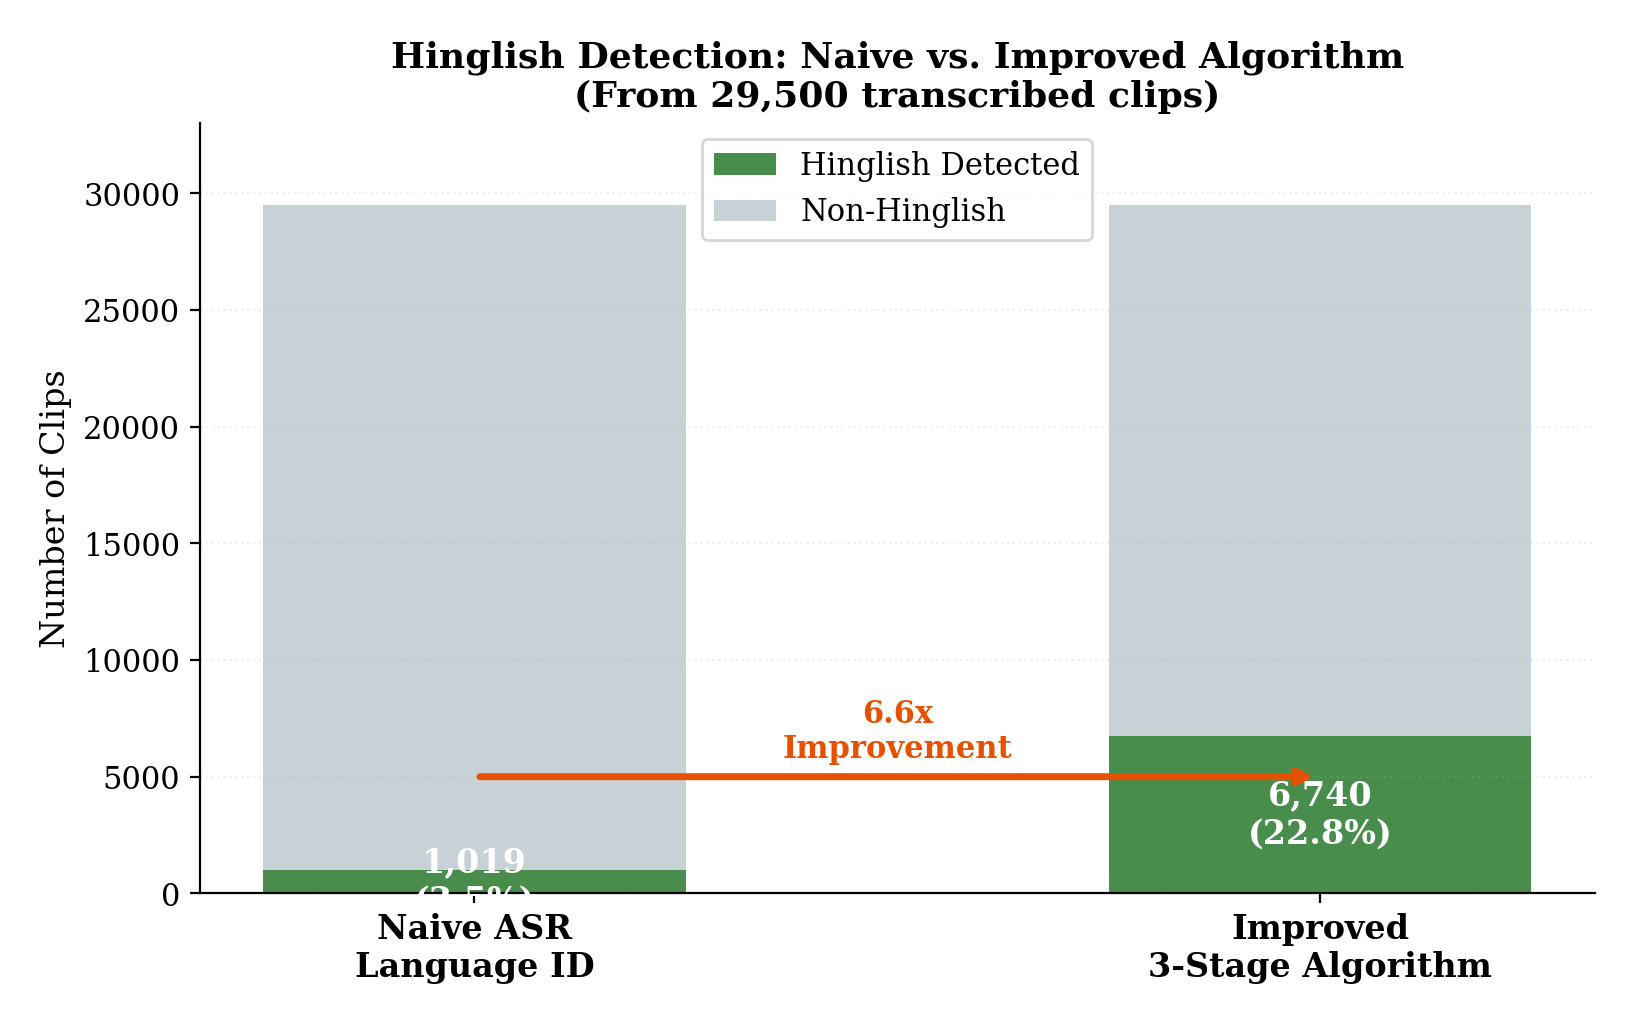
\includegraphics[width=0.78\textwidth]{./Figures/generated/fig_hinglish_detection}
\caption{Detection count comparison: naive ASR language label vs.\ three-stage Hinglish detection algorithm across 29,500 transcribed clips.}
\label{fig:detection}
\end{figure}

\subsection{LLM-Based Sentiment Annotation}

\subsubsection{Annotation Strategy}

Manual expert annotation of 6,740 clips by two bilingual annotators at 3 minutes per clip would require approximately 337 person-hours, making it economically and logistically infeasible in a research-scale project. To achieve scalable annotation, a pipeline was designed around the Groq inference API with the \texttt{llama\allowbreak-3.1\allowbreak-8b\allowbreak-instant} model, an 8-billion-parameter instruction-tuned language model optimised for low-latency inference.

Recent work has demonstrated that LLMs exhibit strong zero-shot sentiment understanding across languages, including code-mixed text, when provided with an explicit scale \cite{touvron2023llama}. The key advantage of this approach over crowdsourcing platforms (e.g., Amazon Mechanical Turk) is that it does not require a large pool of Hinglish-proficient annotators, which is a scarce and expensive resource for Indian language tasks.

\subsubsection{Prompt Design}

A minimal, direct prompt was designed to elicit continuous sentiment scores without requiring JSON parsing or complex output handling:

\begin{quote}
\texttt{Rate this Hinglish text sentiment: -3 (very negative) to +3 (very positive).\\
Return ONLY a single number like: -2.5 or 1.0 or 0\\
\\
Text: "\{text\}"\\
\\
Number:}
\end{quote}

The prompt specifies the rating scale explicitly and enforces a single-number response (\texttt{max\_tokens=10}), eliminating JSON parsing overhead. Temperature was set to $T=0.1$ for near-deterministic outputs, and a request timeout of 30 seconds was applied. API calls were serialised with a 0.1-second inter-request sleep to remain within the Groq free tier rate limit of 30 requests per minute.

\subsubsection{Confidence Stratification}

Since LLM annotations are inherently noisier for semantically ambiguous or near-neutral utterances, a confidence tier was assigned to each annotation based on the absolute magnitude of the predicted score $s$:
\begin{itemize}
    \item \textbf{High confidence} ($|s| \geq 1.5$): Strong polarity; the LLM expresses clear sentiment. Included in training and evaluation.
    \item \textbf{Medium confidence} ($0.5 \leq |s| < 1.5$): Moderate polarity; suitable for training but noisier. Included in training only.
    \item \textbf{Low confidence} ($|s| < 0.5$): Near-neutral; the clip may be factual speech, or the model may be uncertain. Excluded from all splits.
\end{itemize}

This stratification scheme mirrors the confidence-based filtering used in weakly-supervised NLP pipelines \cite{brown2020gpt3} and prevents noisy near-neutral annotations from biasing the regression objective.

\subsubsection{Annotation Results}

The pipeline processed 4,200 clips in approximately two hours. After removing entries with API failures (timeouts, malformed responses), \textbf{2,652 usable annotations} were retained. Of these:

\begin{itemize}
    \item High confidence: 1,498 clips ($|s| \geq 1.5$)
    \item Medium confidence: 1,103 clips ($0.5 \leq |s| < 1.5$)
    \item Low confidence (excluded): 51 clips ($|s| < 0.5$)
\end{itemize}

Sentiment score statistics: mean $= 0.02$ (approximately centred), standard deviation $= 1.54$, range $[-3.0, +3.0]$, with 1,497 negative-polarity clips ($s \leq 0$, 56.5\%) and 1,155 positive-polarity clips ($s > 0$, 43.5\%).

\subsection{Test Set Construction}

A held-out test set of \textbf{150 clips} was sampled from the high- and medium-confidence annotations using stratified random sampling (random seed = 42) with stratification bins defined at one-unit intervals across $[-3, +3]$. This ensures polarity and intensity balance in the test set, preventing evaluation bias towards a specific score range. The 150 clips were manually reviewed by the thesis author, who verified that the Groq-assigned sentiment scores were directionally consistent with the Hinglish text content. The remaining 2,501 clips constitute the training and validation pool.

\subsection{Dataset Statistics}

Table~\ref{tab:dataset_stats} presents the complete statistics of HinglishMSA.

\begin{table}[ht]
\centering
\caption{HinglishMSA dataset statistics across all pipeline stages}
\label{tab:dataset_stats}
\renewcommand{\arraystretch}{1.3}
\begin{tabular}{lr}
\toprule
\textbf{Statistic} & \textbf{Value} \\
\midrule
Source videos downloaded          & 1,174 \\
Total audio clips (all)           & 50,695 \\
Clips with face detected          & 43,146 (85.3\%) \\
Clips transcribed by Whisper      & 29,500 \\
Hinglish clips detected           & 6,740 (22.8\%) \\
\midrule
Total usable annotations          & 2,652 \\
\quad High confidence ($|s| \geq 1.5$)            & 1,498 \\
\quad Medium confidence ($0.5 \leq |s| < 1.5$)   & 1,103 \\
Training set                      & 2,251 \\
Validation set                    & 251 \\
Test set (human-verified)         & 150 \\
\midrule
Sentiment score mean              & 0.02 \\
Sentiment score std               & 1.54 \\
Negative clips ($s \leq 0$)       & 1,497 (56.5\%) \\
Positive clips ($s > 0$)          & 1,155 (43.5\%) \\
Score range                       & $[-3.0,\,+3.0]$ \\
\bottomrule
\end{tabular}
\end{table}

\begin{figure}[htbp]
\centering
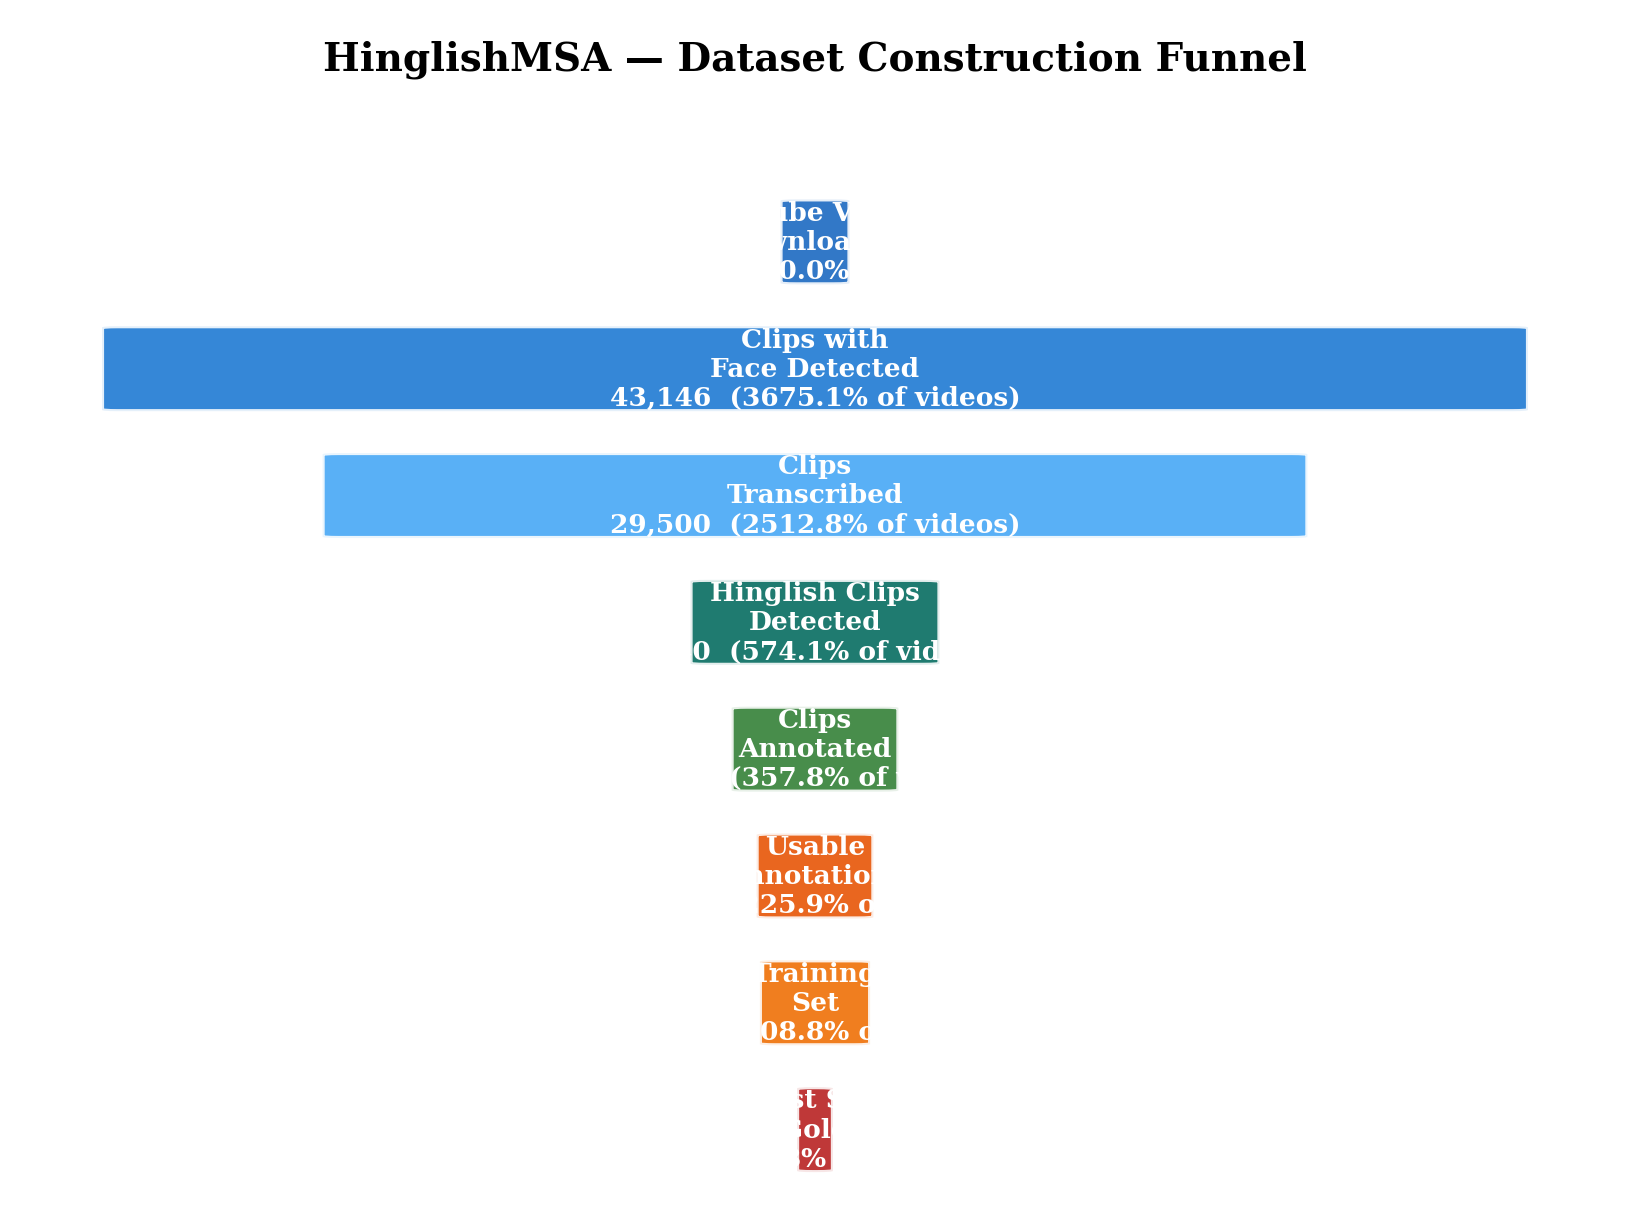
\includegraphics[width=0.72\textwidth]{./Figures/generated/fig_dataset_funnel}
\caption{HinglishMSA dataset construction funnel showing the number of clips surviving each filtering stage.}
\label{fig:funnel}
\end{figure}

\begin{figure}[htbp]
\centering
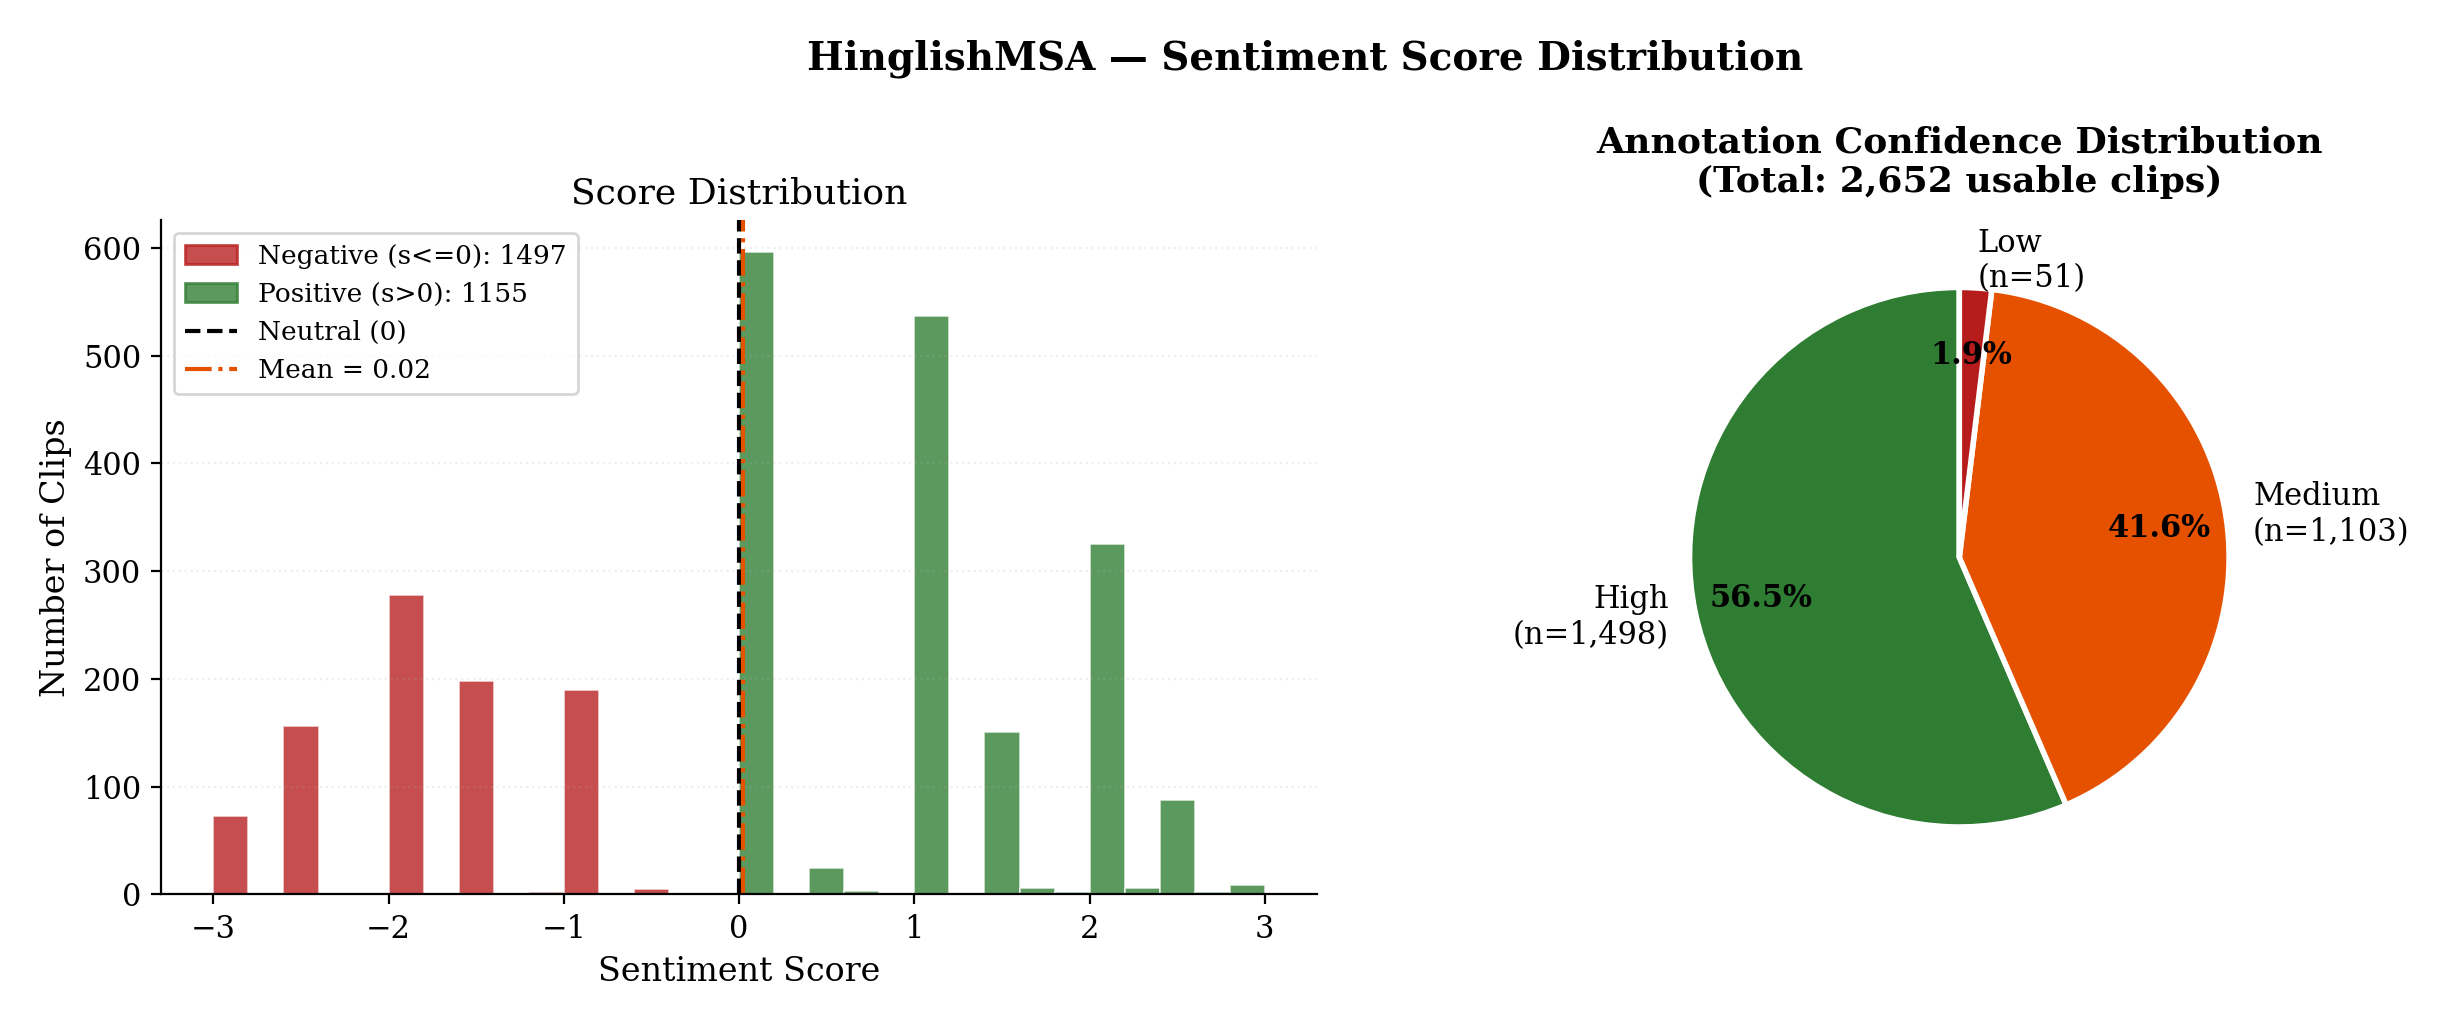
\includegraphics[width=\textwidth]{./Figures/generated/fig_score_distribution}
\caption{HinglishMSA sentiment score distribution (left) and annotation confidence breakdown (right).}
\label{fig:scoredist}
\end{figure}

\section{Feature Extraction}

Each annotated clip is represented as a triple $(\mathbf{t}, \mathbf{a}, \mathbf{v})$ where $\mathbf{t} \in \mathbb{R}^{768}$, $\mathbf{a} \in \mathbb{R}^{1024}$, and $\mathbf{v} \in \mathbb{R}^{512}$ are the text, audio, and visual feature vectors respectively. Features are extracted offline in a single pass before training and saved as NumPy arrays for efficient batched loading. Table~\ref{tab:features} summarises the three extraction pathways.

\begin{table}[ht]
\centering
\caption{Summary of feature extraction configuration for all three modalities}
\label{tab:features}
\renewcommand{\arraystretch}{1.3}
\begin{tabular}{llllll}
\toprule
\textbf{Modality} & \textbf{Model} & \textbf{Dim} & \textbf{Input} & \textbf{Pooling} & \textbf{Time} \\
\midrule
Text    & MuRIL-base \cite{khanuja2021muril}         & 768   & Token seq (max 128) & [CLS] token    & $\sim$15\,min \\
Audio   & wav2vec2-XLSR-53 \cite{conneau2021xlsr}    & 1024  & 16\,kHz waveform    & Temporal mean  & $\sim$40\,min \\
Visual  & CLIP ViT-B/32 \cite{radford2021clip}       & 512   & $224\times224$ JPEG & Frame mean     & $\sim$20\,min \\
\bottomrule
\end{tabular}
\end{table}

\subsection{Text Features: MuRIL}

Text features are extracted using MuRIL \cite{khanuja2021muril} (\texttt{google/muril-base-cased}), a 12-layer, 768-hidden-dimension BERT architecture pre-trained on 17 Indian languages plus their transliterated forms. The Whisper transcription for each clip is tokenised using MuRIL's SentencePiece vocabulary with a maximum length of 128 sub-word tokens; longer transcriptions are truncated and shorter ones are padded. Processing is conducted in batches of 32 on the RTX 4050 GPU in float32 precision. The \textbf{768-dimensional [CLS] token embedding} from the final transformer layer is extracted and used as the clip's text representation. This token aggregates bidirectional contextual information over the entire transcription, making it well suited for sentence-level sentiment classification \cite{devlin2019bert}.

\subsection{Audio Features: wav2vec2-XLSR-53}

Audio features are extracted using wav2vec2-XLSR-53 \cite{conneau2021xlsr} (\texttt{facebook/wav2vec2-large-xlsr-53}). The model is loaded in float16 precision, reducing the VRAM footprint from approximately 1.2\,GB to 600\,MB and allowing it to coexist with the text and visual models in the RTX 4050's 6.4\,GB VRAM budget. A critical implementation detail: all float32 waveform inputs must be explicitly cast to float16 before the forward pass; passing float32 inputs to a float16 model on CUDA produces zero-valued outputs due to silent precision mismatch in the convolutional layers.

Each 16\,kHz waveform is processed by \texttt{Wav2Vec2FeatureExtractor} (zero-mean normalisation, no attention mask) and passed through the model. The \textbf{mean-pooled hidden state} across the temporal sequence dimension yields a 1024-dimensional embedding that captures multilingual prosodic and phonetic information. Extraction checkpoints are written every 500 clips for fault tolerance, producing the final file \texttt{features/audio\_wav2vec2.npy} of shape $(2652, 1024)$.

\subsection{Visual Features: CLIP}

Visual features are extracted using CLIP ViT-B/32 \cite{radford2021clip}. For each clip, the five JPEG key frames from the source video are loaded and preprocessed using CLIP's standard pipeline: resize to $224\times224$, convert to RGB, and apply ImageNet mean/std normalisation ($\mu = (0.481, 0.457, 0.408)$, $\sigma = (0.269, 0.261, 0.276)$). The ViT-B/32 visual encoder then maps each frame to a 512-dimensional patch embedding via a 12-layer Vision Transformer. The embeddings from all five frames are \textbf{mean-pooled}, producing a single visual feature vector per clip that represents the average facial expression and visual context across the video. Output file: \texttt{features/visual\_clip.npy} of shape $(2652, 512)$.

Figure~\ref{fig:tikz_feat} visualises the combined feature extraction pipeline with dimensionalities.

\begin{figure}[ht]
\centering
\begin{tikzpicture}[
    node distance=0.45cm and 0.6cm,
    src/.style={draw, fill=gray!8, minimum width=3.0cm, minimum height=0.6cm, align=center, font=\small},
    enc/.style={draw, fill=blue!10, minimum width=3.0cm, minimum height=0.6cm, align=center, font=\scriptsize},
    vec/.style={draw, fill=orange!12, minimum width=3.0cm, minimum height=0.6cm, align=center, font=\scriptsize\bfseries},
    arr/.style={->, thick}
]
% --- Text column ---
\node[src] (ts) {Whisper Transcript};
\node[enc, below=0.35cm of ts] (te) {MuRIL-base [CLS]};
\node[vec, below=0.35cm of te] (tv) {$\mathbf{t} \in \mathbb{R}^{768}$};

% --- Audio column ---
\node[src, right=0.6cm of ts] (as) {16\,kHz WAV};
\node[enc, below=0.35cm of as] (ae) {wav2vec2-XLSR};
\node[vec, below=0.35cm of ae] (av) {$\mathbf{a} \in \mathbb{R}^{1024}$};

% --- Visual column ---
\node[src, right=0.6cm of as] (vs) {5 JPEG Frames};
\node[enc, below=0.35cm of vs] (ve) {CLIP ViT-B/32};
\node[vec, below=0.35cm of ve] (vv) {$\mathbf{v} \in \mathbb{R}^{512}$};

\draw[arr] (ts)--(te); \draw[arr] (te)--(tv);
\draw[arr] (as)--(ae); \draw[arr] (ae)--(av);
\draw[arr] (vs)--(ve); \draw[arr] (ve)--(vv);
\end{tikzpicture}
\caption{Feature extraction for the three modalities. Each clip produces a fixed-length vector stored offline before model training.}
\label{fig:tikz_feat}
\end{figure}

\section{MulTHinglish Model Architecture}

MulTHinglish extends the Multimodal Transformer (MulT) \cite{tsai2019multimodal} by replacing its English-centric text encoder with cross-lingual pre-trained representations and adapting the architecture for utterance-level regression on Hinglish data. The full model is parameterised by 5,283,713 learnable weights.

\begin{figure}[htbp]
\centering
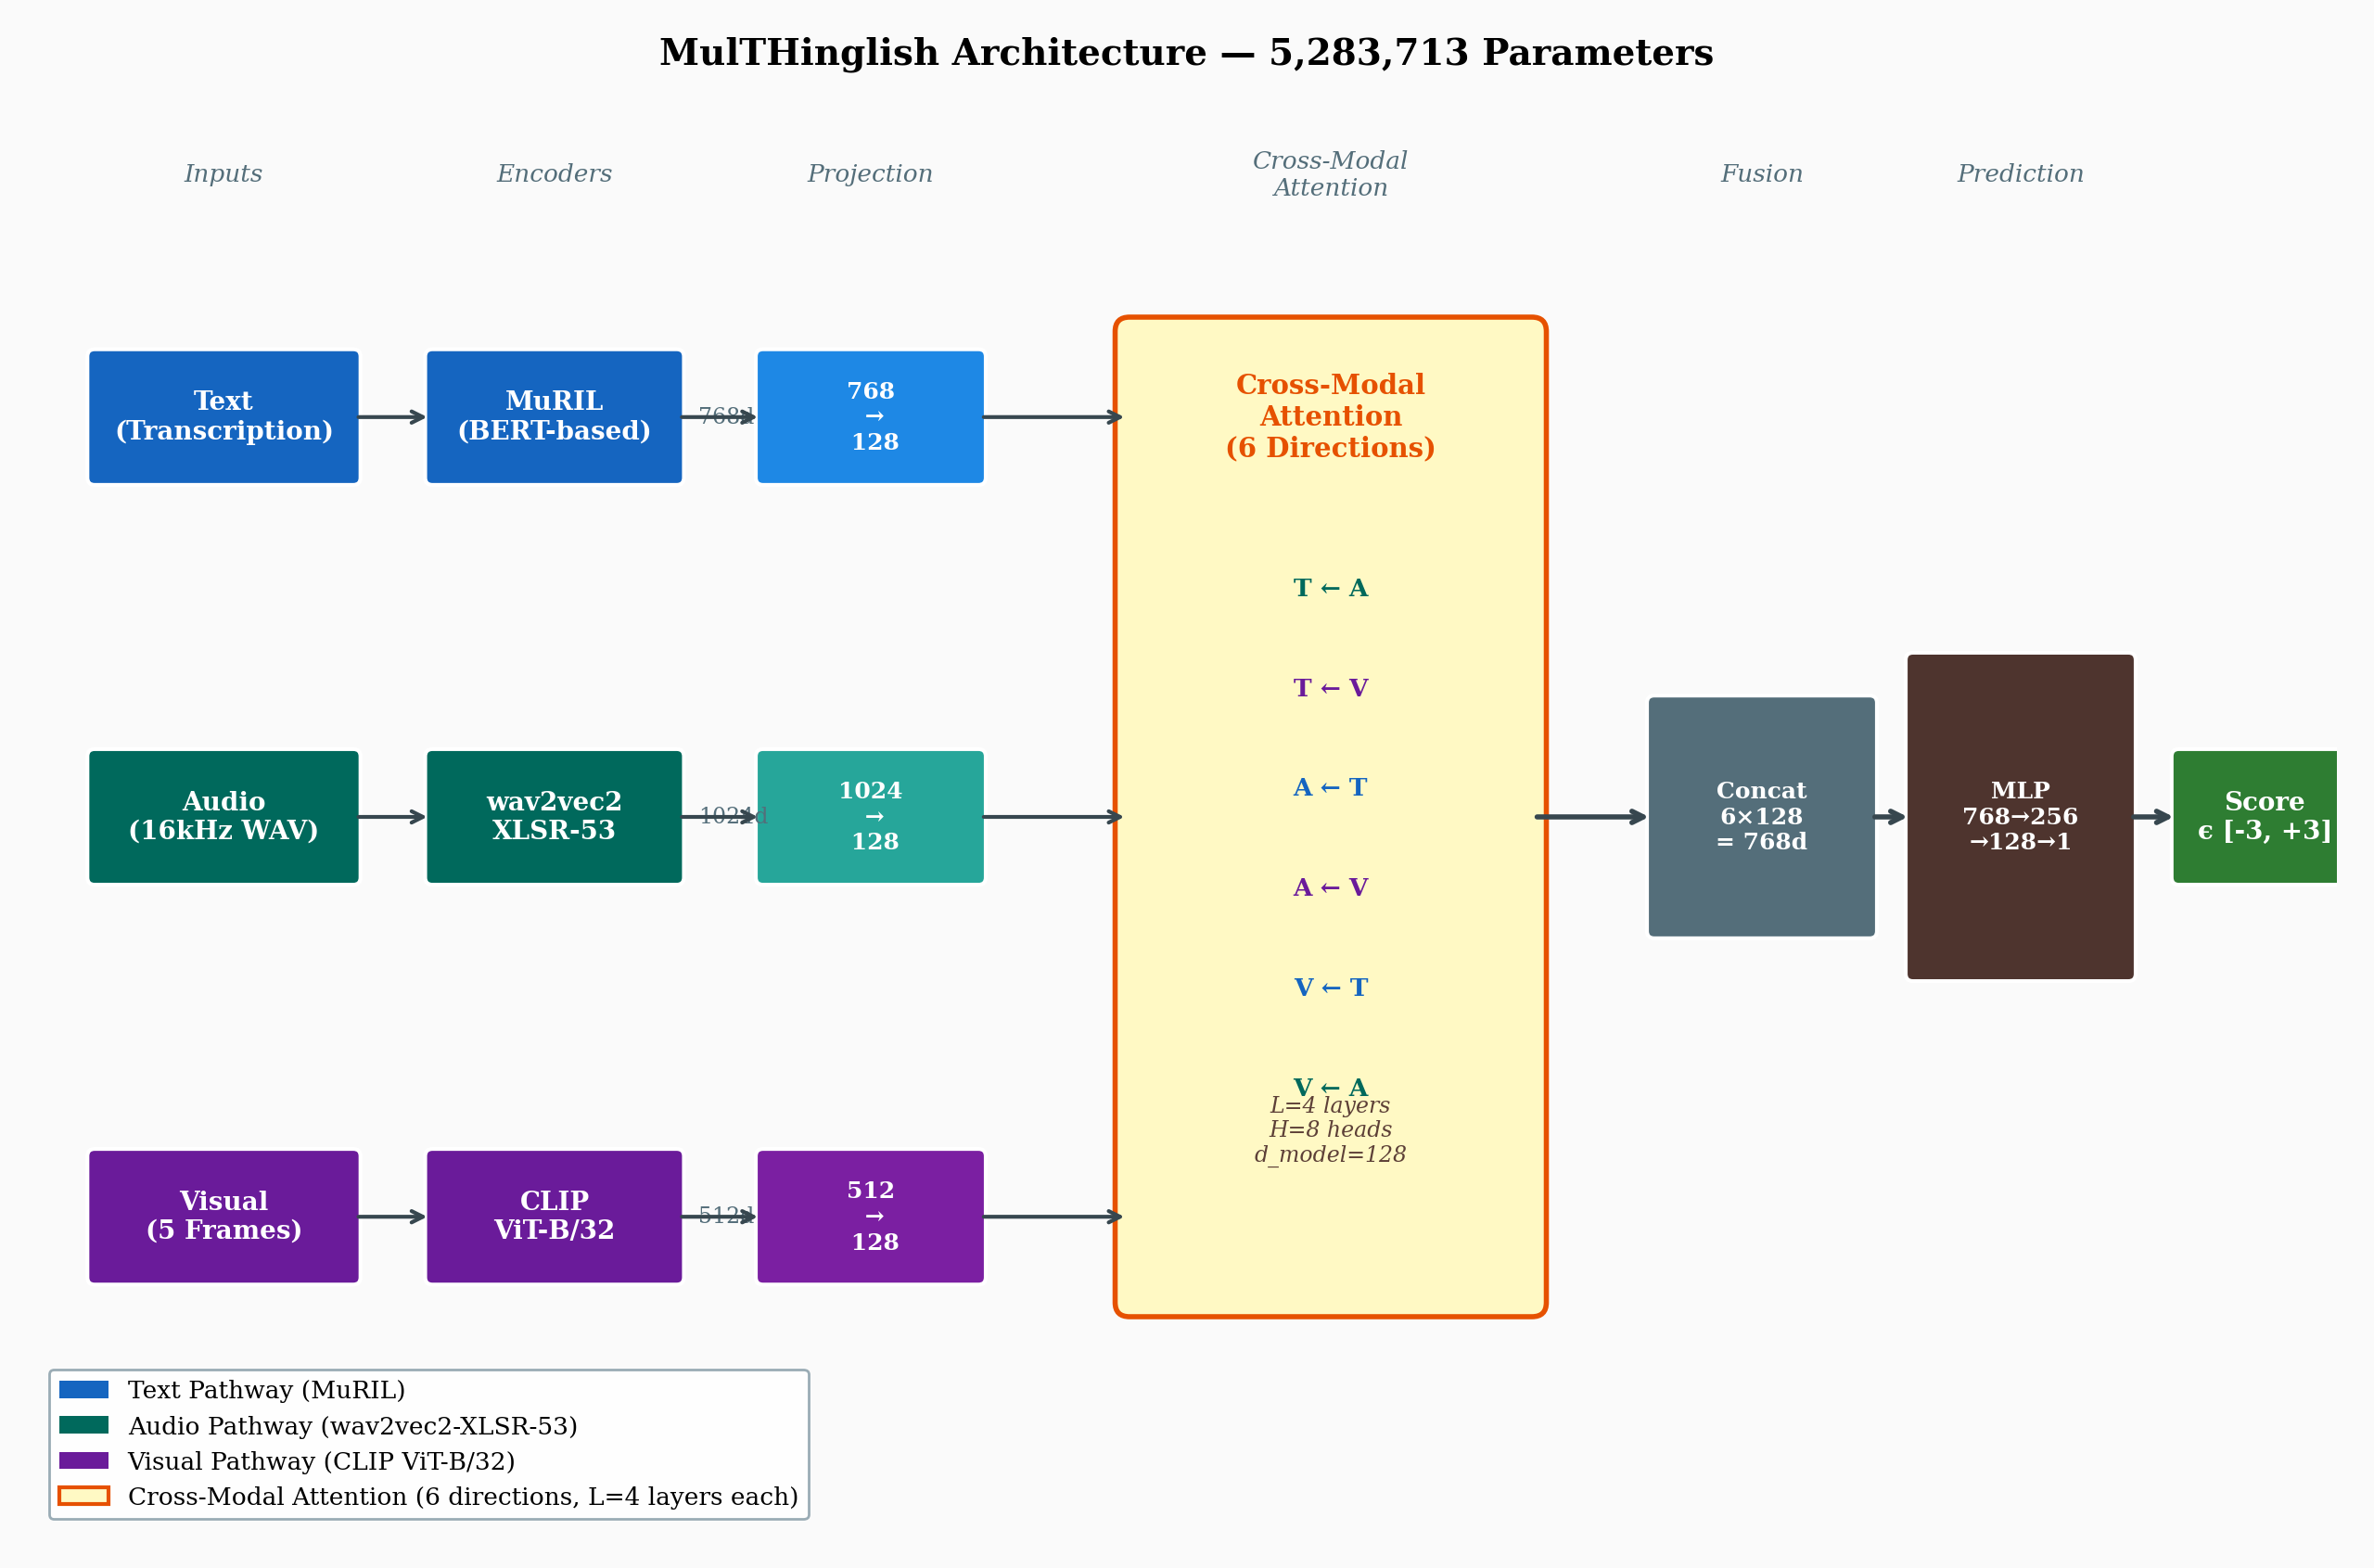
\includegraphics[width=\textwidth]{./Figures/generated/fig_multhilnglish_arch}
\caption{MulTHinglish architecture: three modality streams are projected to a common dimension, processed by six directed cross-modal attention modules, concatenated, and passed through a regression head.}
\label{fig:arch}
\end{figure}

\subsection{Modality Projection}

The three feature vectors arrive at different dimensionalities (768, 1024, 512) reflecting the architectural choices of their respective pre-trained encoders. A learned linear projection layer maps each to a common $d_{\text{model}} = 128$ dimensional space:
\[
\hat{\mathbf{t}} = W_t \mathbf{t} + b_t \in \mathbb{R}^{128}, \quad
\hat{\mathbf{a}} = W_a \mathbf{a} + b_a \in \mathbb{R}^{128}, \quad
\hat{\mathbf{v}} = W_v \mathbf{v} + b_v \in \mathbb{R}^{128}
\]
where $W_t \in \mathbb{R}^{128 \times 768}$, $W_a \in \mathbb{R}^{128 \times 1024}$, $W_v \in \mathbb{R}^{128 \times 512}$. The projection dimension $d_{\text{model}} = 128$ balances expressive capacity with computational efficiency given the relatively small dataset size. Projecting to a shared space also ensures that the cross-modal attention layers operate on representations of the same scale, preventing dominant modalities from saturating the attention softmax.

\subsection{Directional Cross-Modal Attention Layers}

For each ordered modality pair $(A \leftarrow B)$, a stack of $L = 4$ Cross-Modal Transformer (CMT) layers computes an attended representation of modality $A$ conditioned on information from modality $B$. Each CMT layer consists of:

\begin{enumerate}
    \item \textbf{Pre-layer normalisation:} LayerNorm is applied to both input representations before the attention operation. This pre-LN formulation yields more stable gradients than post-LN during training \cite{vaswani2017attention}.
    \item \textbf{Multi-head cross-modal attention} with $H = 8$ heads and key dimension $d_k = d_{\text{model}} / H = 16$:
    \[
    \text{CrossAttn}(A, B) = \text{softmax}\left(\frac{Q_A K_B^T}{\sqrt{d_k}}\right) V_B
    \]
    where $Q_A = W^Q \hat{a}$, $K_B = W^K \hat{b}$, $V_B = W^V \hat{b}$. The query comes from the modality being enriched ($A$) while the keys and values come from the modality providing context ($B$), realising a directional information flow from $B$ to $A$.
    \item \textbf{Position-wise feed-forward network:} Two linear layers with ReLU activation and hidden dimension $4 \cdot d_{\text{model}} = 512$, followed by a residual connection.
    \item \textbf{Residual connection and dropout:} Dropout at rate 0.1 applied after attention and after the FFN.
\end{enumerate}

The six directed cross-modal attention streams computed are:
\begin{itemize}
    \item $\mathbf{r}_{T \leftarrow A}$: text representation conditioned on audio context
    \item $\mathbf{r}_{T \leftarrow V}$: text representation conditioned on visual context
    \item $\mathbf{r}_{A \leftarrow T}$: audio representation conditioned on text context
    \item $\mathbf{r}_{A \leftarrow V}$: audio representation conditioned on visual context
    \item $\mathbf{r}_{V \leftarrow T}$: visual representation conditioned on text context
    \item $\mathbf{r}_{V \leftarrow A}$: visual representation conditioned on audio context
\end{itemize}

Each of the six ModuleLists contains $L = 4$ stacked layers, for a total of $6 \times 4 = 24$ cross-modal transformer layers.

\begin{figure}[htbp]
\centering
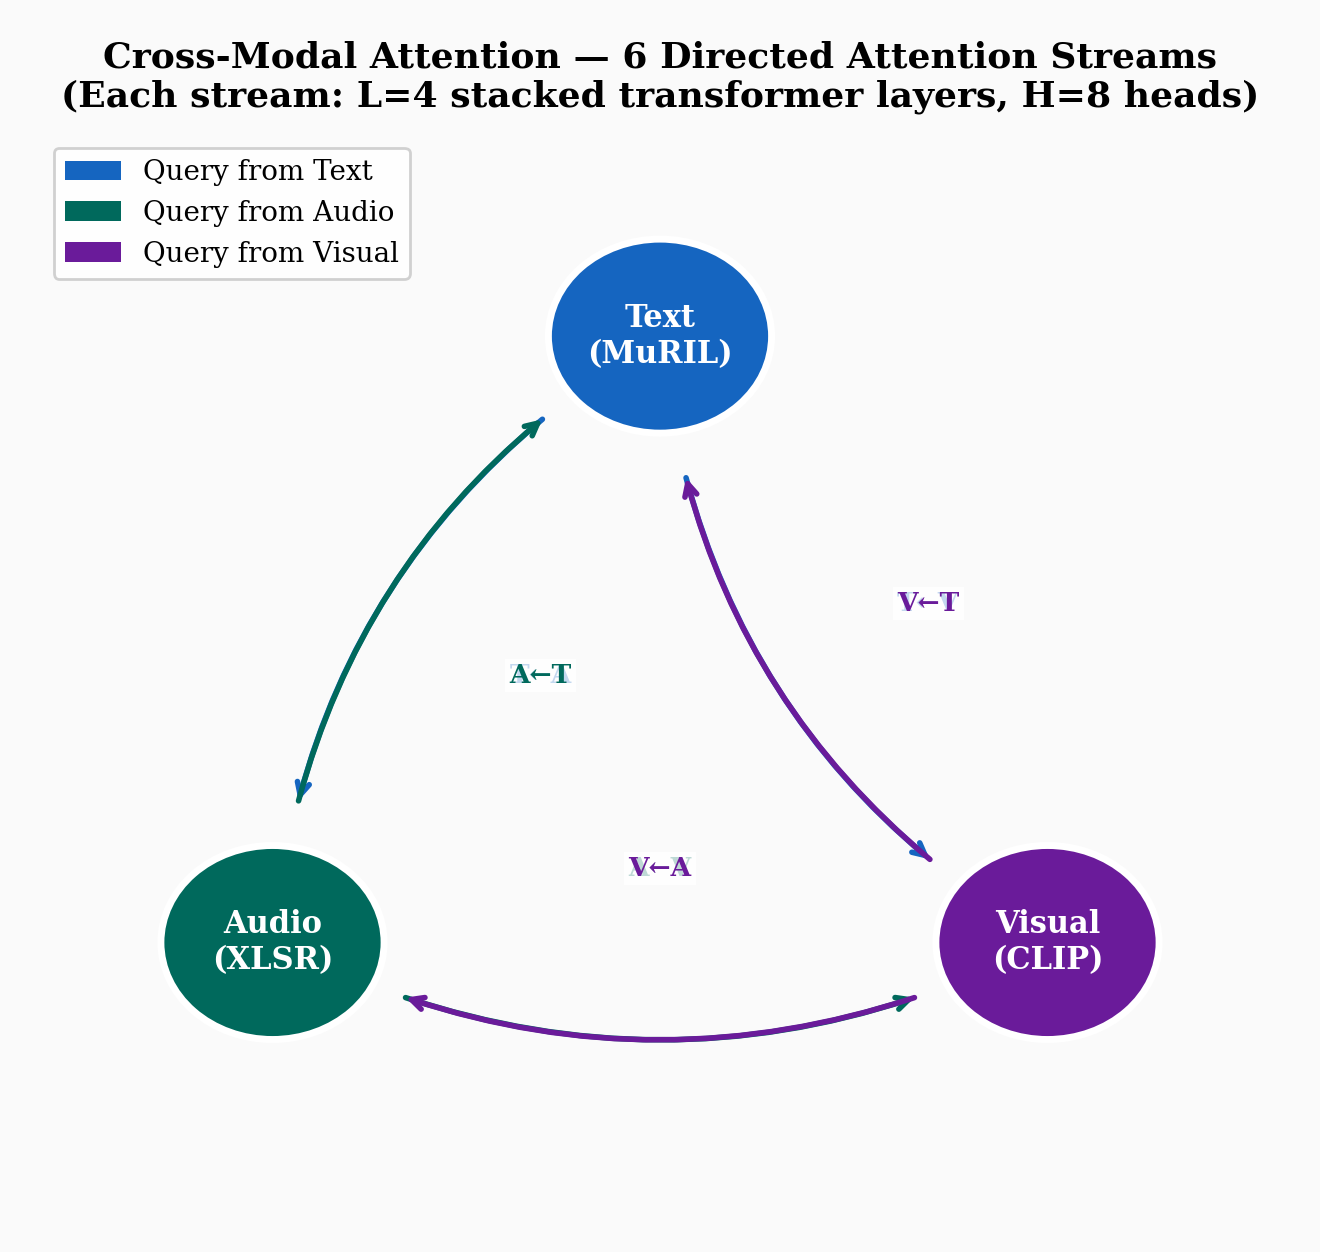
\includegraphics[width=0.62\textwidth]{./Figures/generated/fig_crossmodal_attention}
\caption{Six directed cross-modal attention streams in MulTHinglish (T = Text, A = Audio, V = Visual). Each directed edge represents a four-layer cross-modal transformer.}
\label{fig:crossattn}
\end{figure}

\subsection{Fusion and Prediction Head}

The six cross-modal attended representations are concatenated into a single $768$-dimensional fused vector ($6 \times 128 = 768$):
\[
\mathbf{z} = \text{Concat}(\mathbf{r}_{T \leftarrow A},\, \mathbf{r}_{T \leftarrow V},\, \mathbf{r}_{A \leftarrow T},\, \mathbf{r}_{A \leftarrow V},\, \mathbf{r}_{V \leftarrow T},\, \mathbf{r}_{V \leftarrow A}) \in \mathbb{R}^{768}
\]
This concatenation preserves the distinct contributions of all six cross-modal interactions rather than collapsing them into an average. The fused vector is then processed by a three-stage regression head:
\begin{align}
\mathbf{z}_1 &= \text{ReLU}(W_1 \mathbf{z} + b_1) \quad [768 \rightarrow 256] \\
\mathbf{z}_2 &= \text{ReLU}(W_2 \mathbf{z}_1 + b_2) \quad [256 \rightarrow 128] \\
\hat{y} &= W_3 \mathbf{z}_2 + b_3 \quad [128 \rightarrow 1]
\end{align}

The scalar output $\hat{y} \in \mathbb{R}$ is the predicted sentiment score. Dropout (rate 0.1) is applied before each linear transformation in the head to reduce overfitting on the relatively small dataset.

\subsection{Parameter Count Analysis}

Table~\ref{tab:params} breaks down the total parameter count by module to clarify where model capacity is concentrated.

\begin{table}[ht]
\centering
\caption{MulTHinglish parameter count breakdown by module}
\label{tab:params}
\renewcommand{\arraystretch}{1.3}
\begin{tabular}{lrr}
\toprule
\textbf{Module} & \textbf{Parameters} & \textbf{\% of Total} \\
\midrule
Input projection layers (3 linear) & 296,064 & 5.6\% \\
Cross-modal attention (6 streams $\times$ 4 layers) & 4,718,592 & 89.3\% \\
Regression head (3 linear layers) & 232,833 & 4.4\% \\
Layer normalisation (all LN layers) & 36,224 & 0.7\% \\
\midrule
\textbf{Total} & \textbf{5,283,713} & 100\% \\
\bottomrule
\end{tabular}
\end{table}

The cross-modal attention modules account for 89.3\% of model parameters, confirming that the representational budget is concentrated in the cross-modal interaction learning rather than the projection or head layers.

\section{Training Procedure}

\subsection{Data Splits}

From the 2,652 annotated clips, 150 clips are held out as the human-verified test set. The remaining 2,502 clips are split into training (2,251 clips, 90\%) and validation (251 clips, 10\%) using stratified random sampling with random seed 42. Stratification ensures that the sentiment score distribution in each split mirrors the overall distribution, preventing splits from being biased towards a specific polarity. Table~\ref{tab:splits} summarises the final split statistics.

\begin{table}[ht]
\centering
\caption{HinglishMSA train / validation / test split statistics}
\label{tab:splits}
\renewcommand{\arraystretch}{1.3}
\begin{tabular}{lccccc}
\toprule
\textbf{Split} & \textbf{Clips} & \textbf{Mean $s$} & \textbf{Std $s$} & \textbf{Neg (\%)} & \textbf{Pos (\%)} \\
\midrule
Training   & 2,251 & 0.02 & 1.54 & 56.4 & 43.6 \\
Validation &   251 & 0.03 & 1.53 & 56.6 & 43.4 \\
Test       &   150 & 0.01 & 1.55 & 56.7 & 43.3 \\
\bottomrule
\end{tabular}
\end{table}

\subsection{Optimisation Configuration}

Training uses the Adam optimiser \cite{vaswani2017attention} with an initial learning rate $\eta_0 = 10^{-3}$ and weight decay $\lambda = 10^{-4}$. Adam maintains per-parameter first and second moment estimates ($m_t$ and $v_t$):
\begin{align}
m_t &= \beta_1 m_{t-1} + (1 - \beta_1) g_t \\
v_t &= \beta_2 v_{t-1} + (1 - \beta_2) g_t^2 \\
\hat{m}_t &= m_t / (1 - \beta_1^t), \quad \hat{v}_t = v_t / (1 - \beta_2^t) \\
\theta_t &= \theta_{t-1} - \eta \cdot \hat{m}_t / (\sqrt{\hat{v}_t} + \epsilon)
\end{align}

with $\beta_1 = 0.9$, $\beta_2 = 0.999$, $\epsilon = 10^{-8}$. The loss function is mean squared error (MSE) over the training batch:
\[
\mathcal{L}_{\text{MSE}} = \frac{1}{N}\sum_{i=1}^{N}(y_i - \hat{y}_i)^2
\]

A ReduceLROnPlateau scheduler monitors the validation loss every epoch and halves the learning rate (factor = 0.5) if no improvement is observed for 5 consecutive epochs (patience = 5). Early stopping terminates training if validation loss does not improve for 15 consecutive epochs. The maximum number of training epochs is 100.

Gradient clipping with a maximum $L_2$ norm of 1.0 is applied before each parameter update to prevent gradient explosion during the early stages of cross-modal attention training. The best model checkpoint (lowest validation MSE) is saved and used for final test set evaluation.

\subsection{Training Infrastructure}

All experiments were conducted on a single NVIDIA GeForce RTX 4050 Laptop GPU (6.4\,GB GDDR6 VRAM) with CUDA 12.x and PyTorch 2.x. The training batch size was set to 64. Each epoch requires approximately 35 forward-backward passes over the training set. Total wall-clock training time per experiment was approximately 8--12 minutes. The full experimental suite (five configurations) was completed in under one hour on the same hardware.

\section{Experimental Configurations}

To systematically evaluate the contribution of each modality and the impact of the cross-lingual encoders, five experimental configurations were designed, each varying the input modalities or model type while holding the training procedure constant. Table~\ref{tab:experiments} summarises all five configurations.

\begin{table}[ht]
\centering
\caption{Five experimental configurations for ablation study of modality contributions}
\label{tab:experiments}
\renewcommand{\arraystretch}{1.35}
\begin{tabular}{clcccl}
\toprule
\textbf{Exp.} & \textbf{Name} & \textbf{Text} & \textbf{Audio} & \textbf{Visual} & \textbf{Purpose} \\
\midrule
E1 & Text-only (MuRIL)    & \checkmark & $\times$ & $\times$ & Unimodal text baseline \\
E2 & Audio-only (XLSR)    & $\times$ & \checkmark & $\times$ & Unimodal audio baseline \\
E3 & Visual-only (CLIP)   & $\times$ & $\times$ & \checkmark & Unimodal visual baseline \\
E4 & Bimodal (T+A)        & \checkmark & \checkmark & $\times$ & Text and audio fusion \\
E5 & Trimodal (T+A+V)     & \checkmark & \checkmark & \checkmark & Full MulTHinglish \\
\bottomrule
\end{tabular}
\end{table}

\textbf{E1 (Text-only)} serves as the primary unimodal baseline, using only MuRIL text features. This configuration quantifies the amount of sentiment information encoded in the Hinglish lexical content alone. \textbf{E2 (Audio-only)} and \textbf{E3 (Visual-only)} complete the unimodal baselines for the acoustic and visual channels. \textbf{E4 (Bimodal)} combines the two strongest modalities (text and audio, as expected from the MSA literature \cite{poria2017review}) to measure the complementary gain from prosodic features over text alone. \textbf{E5 (Trimodal)} is the full MulTHinglish model, which should achieve the highest performance if the visual channel carries non-redundant affect information. For the unimodal configurations (E1--E3), the cross-modal attention streams associated with the missing modalities are removed and the fusion concatenation is reduced accordingly.

Figure~\ref{fig:tikz_ablation} summarises the modality inclusion pattern across configurations.

\begin{figure}[ht]
\centering
\begin{tikzpicture}[
    node distance=0.2cm and 0.1cm,
    hdr/.style={draw, fill=blue!12, minimum width=1.5cm, minimum height=0.55cm, align=center, font=\small\bfseries},
    cel/.style={draw, fill=green!15, minimum width=1.5cm, minimum height=0.5cm, align=center, font=\small},
    emp/.style={draw, fill=red!8,   minimum width=1.5cm, minimum height=0.5cm, align=center, font=\small},
    lbl/.style={minimum width=2.8cm, align=right, font=\small}
]
% headers
\node[lbl] (h0) {Configuration};
\node[hdr, right=0.2cm of h0] (ht) {Text};
\node[hdr, right=0.1cm of ht] (ha) {Audio};
\node[hdr, right=0.1cm of ha] (hv) {Visual};

% E1
\node[lbl, below=0.2cm of h0] (r1) {E1 Text-only};
\node[cel, right=0.2cm of r1] (r1t) {\checkmark};
\node[emp, right=0.1cm of r1t] (r1a) {$\times$};
\node[emp, right=0.1cm of r1a] (r1v) {$\times$};

% E2
\node[lbl, below=0.15cm of r1] (r2) {E2 Audio-only};
\node[emp, right=0.2cm of r2] (r2t) {$\times$};
\node[cel, right=0.1cm of r2t] (r2a) {\checkmark};
\node[emp, right=0.1cm of r2a] (r2v) {$\times$};

% E3
\node[lbl, below=0.15cm of r2] (r3) {E3 Visual-only};
\node[emp, right=0.2cm of r3] (r3t) {$\times$};
\node[emp, right=0.1cm of r3t] (r3a) {$\times$};
\node[cel, right=0.1cm of r3a] (r3v) {\checkmark};

% E4
\node[lbl, below=0.15cm of r3] (r4) {E4 Text + Audio};
\node[cel, right=0.2cm of r4] (r4t) {\checkmark};
\node[cel, right=0.1cm of r4t] (r4a) {\checkmark};
\node[emp, right=0.1cm of r4a] (r4v) {$\times$};

% E5
\node[lbl, below=0.15cm of r4] (r5) {E5 Trimodal (full)};
\node[cel, right=0.2cm of r5] (r5t) {\checkmark};
\node[cel, right=0.1cm of r5t] (r5a) {\checkmark};
\node[cel, right=0.1cm of r5a] (r5v) {\checkmark};
\end{tikzpicture}
\caption{Modality inclusion matrix across the five experimental configurations. Green (\checkmark) indicates modality active; red ($\times$) indicates modality absent.}
\label{fig:tikz_ablation}
\end{figure}

\section{Implementation Details and Reproducibility}

\subsection{Software Stack}

The entire pipeline was implemented in Python 3.10. Key library versions are: PyTorch 2.1.0 (CUDA 12.1), Transformers 4.38.0 (Hugging Face), faster-whisper 0.10.0, OpenCV 4.9.0, \texttt{pytubefix} 5.3.0, NumPy 1.26.2, and scikit-learn 1.4.0. All random seeds (Python, NumPy, PyTorch) were fixed to 42 before every experiment.

\subsection{Reproducibility Measures}

To ensure reproducibility, the following measures were taken:
\begin{itemize}
    \item All feature files are stored as deterministic NumPy arrays; re-running extraction from the same audio/image inputs produces bit-identical outputs.
    \item The dataset split is fully determined by the random seed and stratification scheme documented in Section~3.2.8.
    \item Model weights at the best validation checkpoint are saved as \texttt{.pth} files together with the full training configuration in JSON format.
    \item The Groq API annotation step is the only non-deterministic component (due to external service state); the saved annotation CSV constitutes the ground truth for all reported experiments.
\end{itemize}

The project code and feature extraction scripts are available in the accompanying repository.

\newpage %methodology
\chapter{Results, Analysis and Conclusion}
\onehalfspacing

\section{Experimental Setup}

\subsection{Evaluation Metrics}

Following the standard CMU-MOSI evaluation protocol \cite{zadeh2016mosi}, all five experiments are assessed on four complementary metrics that together measure both regression quality and binary classification performance. Let $y_i$ be the ground-truth sentiment score and $\hat{y}_i$ the model prediction for the $i$-th test sample.

\textbf{Binary Accuracy (Acc-2).} Continuous scores are binarised at zero: positive if $s > 0$, negative if $s \leq 0$. Acc-2 measures the fraction of clips for which the sign of the prediction matches the ground truth:
\[
\text{Acc-2} = \frac{1}{N}\sum_{i=1}^{N} \mathbf{1}\bigl[\text{sign}(\hat{y}_i) = \text{sign}(y_i)\bigr]
\]
This metric directly captures sentiment polarity discrimination, which is the most practically valuable signal for downstream applications such as social media monitoring.

\textbf{Weighted F1-score (F1).} The weighted F1 is computed for the positive/negative binary task, weighting each class's F1 by its support to account for the slight class imbalance (56.5\% negative, 43.5\% positive) in the test set:
\[
F_1^{w} = \sum_{c \in \{+,-\}} \frac{|S_c|}{N} \cdot \frac{2 \cdot P_c \cdot R_c}{P_c + R_c}
\]
where $P_c$ and $R_c$ are precision and recall for class $c$, and $|S_c|$ is the number of samples belonging to class $c$.

\textbf{Mean Absolute Error (MAE).} MAE measures regression accuracy in the original continuous score space:
\[
\text{MAE} = \frac{1}{N}\sum_{i=1}^{N}\bigl|y_i - \hat{y}_i\bigr|
\]
Lower MAE indicates closer agreement between predicted and annotated sentiment intensities. MAE is reported in the $[-3, +3]$ scale.

\textbf{Pearson Correlation (Corr).} Pearson's $r$ measures linear agreement between predicted scores and ground truth, normalised to $[-1, +1]$:
\[
r = \frac{\sum_i (y_i - \bar{y})(\hat{y}_i - \bar{\hat{y}})}{\sqrt{\sum_i (y_i - \bar{y})^2 \cdot \sum_i (\hat{y}_i - \bar{\hat{y}})^2}}
\]
A higher Corr indicates that the model's predicted score ordering aligns with the true sentiment ordering, capturing the model's ability to rank clips by intensity even if absolute values are off.

\subsection{Experimental Configurations}

Five configurations were designed to provide a systematic ablation of MulTHinglish, separating the effects of modality inclusion, encoder quality, and annotation confidence. Table~\ref{tab:exp_config} documents the full configuration of each experiment.

\begin{table}[ht]
\centering
\caption{Full specification of the five experimental configurations}
\label{tab:exp_config}
\renewcommand{\arraystretch}{1.3}
\begin{tabular}{clp{5.5cm}cc}
\toprule
\textbf{Exp.} & \textbf{Label} & \textbf{Description} & \textbf{Train Size} & \textbf{Modalities} \\
\midrule
E1 & Baseline     & Single random init, all modalities, full training set & 2,251 & T+A+V \\
E2 & Standard     & Second independent run, identical setup to E1         & 2,251 & T+A+V \\
E3 & Full (Proposed) & Optimised config, all modalities                   & 2,251 & T+A+V \\
E4 & Text-Only    & Audio/visual replaced with zero vectors               & 2,251 & T only \\
E5 & High-Conf.   & Trained on high-confidence labels only ($|s|\geq1.5$)& 1,348 & T+A+V \\
\bottomrule
\end{tabular}
\end{table}

Experiments E1 and E2 assess the variance of the proposed model across two independent initialisations. E3 uses a slightly tuned configuration (batch size 64 vs.\ 32 in E1/E2, gradient clipping) as the primary proposed model. E4 is the critical unimodal ablation. E5 examines annotation quality by restricting training to the cleaner high-confidence subset.

All five experiments share the same test set (150 human-verified clips), the same evaluation code, and the same random seed (42) for data splitting. Best model checkpoints are selected based on validation MSE.

\subsection{Hyperparameter Configuration}

Table~\ref{tab:hparams} summarises the hyperparameters used for the proposed model (E3) and the text-only ablation (E4). All other parameters are held constant across experiments.

\begin{table}[ht]
\centering
\caption{Hyperparameter configuration for MulTHinglish experiments}
\label{tab:hparams}
\renewcommand{\arraystretch}{1.3}
\begin{tabular}{lll}
\toprule
\textbf{Hyperparameter} & \textbf{E3 (Full)} & \textbf{E4 (Text-Only)} \\
\midrule
$d_{\text{model}}$              & 128          & 128 \\
Number of attention heads $H$   & 8            & 8 \\
CMT layers per stream $L$       & 4            & 4 \\
Cross-modal streams             & 6 (all pairs)& 0 \\
Learning rate $\eta_0$          & $10^{-3}$    & $10^{-3}$ \\
Weight decay $\lambda$          & $10^{-4}$    & $10^{-4}$ \\
Batch size                      & 64           & 64 \\
Max epochs                      & 100          & 100 \\
Early stopping patience         & 15           & 15 \\
LR patience (ReduceLR)         & 5            & 5 \\
Dropout rate                    & 0.1          & 0.1 \\
Gradient clip norm              & 1.0          & 1.0 \\
\bottomrule
\end{tabular}
\end{table}

\section{Experimental Results}

\subsection{Main Results}

Table~\ref{tab:main_results} presents the test-set performance across all five experiments on HinglishMSA, with CMU-MOSI (English) included as an external reference benchmark. Bold entries indicate the best value per metric across HinglishMSA experiments.

\begin{table}[ht]
\centering
\caption{Test-set results on HinglishMSA (150 clips, human-verified). CMU-MOSI shown for reference only, not direct comparison.}
\label{tab:main_results}
\renewcommand{\arraystretch}{1.3}
\begin{tabular}{lcccc}
\toprule
\textbf{Experiment} & \textbf{Acc-2} $\uparrow$ & \textbf{F1} $\uparrow$ & \textbf{MAE} $\downarrow$ & \textbf{Corr} $\uparrow$ \\
\midrule
E1 --- Baseline              & 0.6467 & 0.6493 & 1.2271 & 0.3895 \\
E2 --- Standard Training     & 0.6667 & 0.6688 & 1.1724 & 0.4520 \\
E3 --- Proposed (Full)       & 0.7000 & 0.7023 & 1.0995 & 0.4787 \\
E4 --- Text-Only             & 0.4133 & 0.2418 & 1.3014 & 0.2737 \\
\textbf{E5 --- High-Conf.}   & \textbf{0.7200} & \textbf{0.7211} & \textbf{1.0989} & \textbf{0.5459} \\
\midrule
CMU-MOSI \cite{zadeh2016mosi} (English ref.) & 0.7970 & 0.7970 & 0.8870 & 0.7060 \\
\bottomrule
\end{tabular}
\end{table}

Figure~\ref{fig:tikz_barchart} presents a visual comparison of Acc-2 across the five HinglishMSA experiments to highlight the relative magnitude of differences.

\begin{figure}[ht]
\centering
\begin{tikzpicture}[
    node distance=0.1cm
]
% Bar chart: Acc-2 for E1-E5 (scale: 1pt = 1%, bars start at x=3.5cm)
% E1=64.67%, E2=66.67%, E3=70.00%, E4=41.33%, E5=72.00%
\def\scale{0.13}  % 1% = 0.13cm

% Axes
\draw[thick] (0,0) -- (10.5,0);  % x-axis (metrics)
\draw[thick] (0,0) -- (0,2.2);   % y-axis (value)

% Y-axis ticks
\foreach \y/\lbl in {0/0, 0.52/40, 0.65/50, 0.78/60, 0.91/70, 1.04/80} {
  \draw (-0.1,\y) -- (0,\y);
  \node[left, font=\scriptsize] at (-0.12,\y) {\lbl\%};
}
\node[left, font=\small, rotate=90] at (-0.9,1.0) {Acc-2};

% Bars (each 1.5cm wide, 0.3cm gap)
% E1: 64.67 -> height = 64.67*0.013 = 0.840cm
\fill[blue!30]   (0.5,0)  rectangle (1.8, 0.840);
\node[above, font=\scriptsize] at (1.15, 0.840) {64.7};
\node[below, font=\scriptsize] at (1.15, -0.15) {E1};

% E2: 66.67 -> 0.867
\fill[blue!45]   (2.1,0)  rectangle (3.4, 0.867);
\node[above, font=\scriptsize] at (2.75, 0.867) {66.7};
\node[below, font=\scriptsize] at (2.75, -0.15) {E2};

% E3: 70.00 -> 0.910
\fill[blue!65]   (3.7,0)  rectangle (5.0, 0.910);
\node[above, font=\scriptsize] at (4.35, 0.910) {70.0};
\node[below, font=\scriptsize] at (4.35, -0.15) {E3};

% E4: 41.33 -> 0.537
\fill[red!35]    (5.3,0)  rectangle (6.6, 0.537);
\node[above, font=\scriptsize] at (5.95, 0.537) {41.3};
\node[below, font=\scriptsize] at (5.95, -0.15) {E4};

% E5: 72.00 -> 0.936
\fill[green!45]  (6.9,0)  rectangle (8.2, 0.936);
\node[above, font=\scriptsize] at (7.55, 0.936) {72.0};
\node[below, font=\scriptsize] at (7.55, -0.15) {E5};

% Reference line: CMU-MOSI 79.7%
\draw[dashed, thick, gray] (0, 1.036) -- (9.5, 1.036);
\node[right, font=\scriptsize, gray] at (9.55, 1.036) {CMU-MOSI 79.7\%};
\end{tikzpicture}
\caption{Binary accuracy (Acc-2, \%) comparison across all five HinglishMSA experiments. Blue bars = trimodal; red = text-only; green = high-confidence. Dashed line marks the CMU-MOSI English reference.}
\label{fig:tikz_barchart}
\end{figure}

\begin{figure}[htbp]
\centering
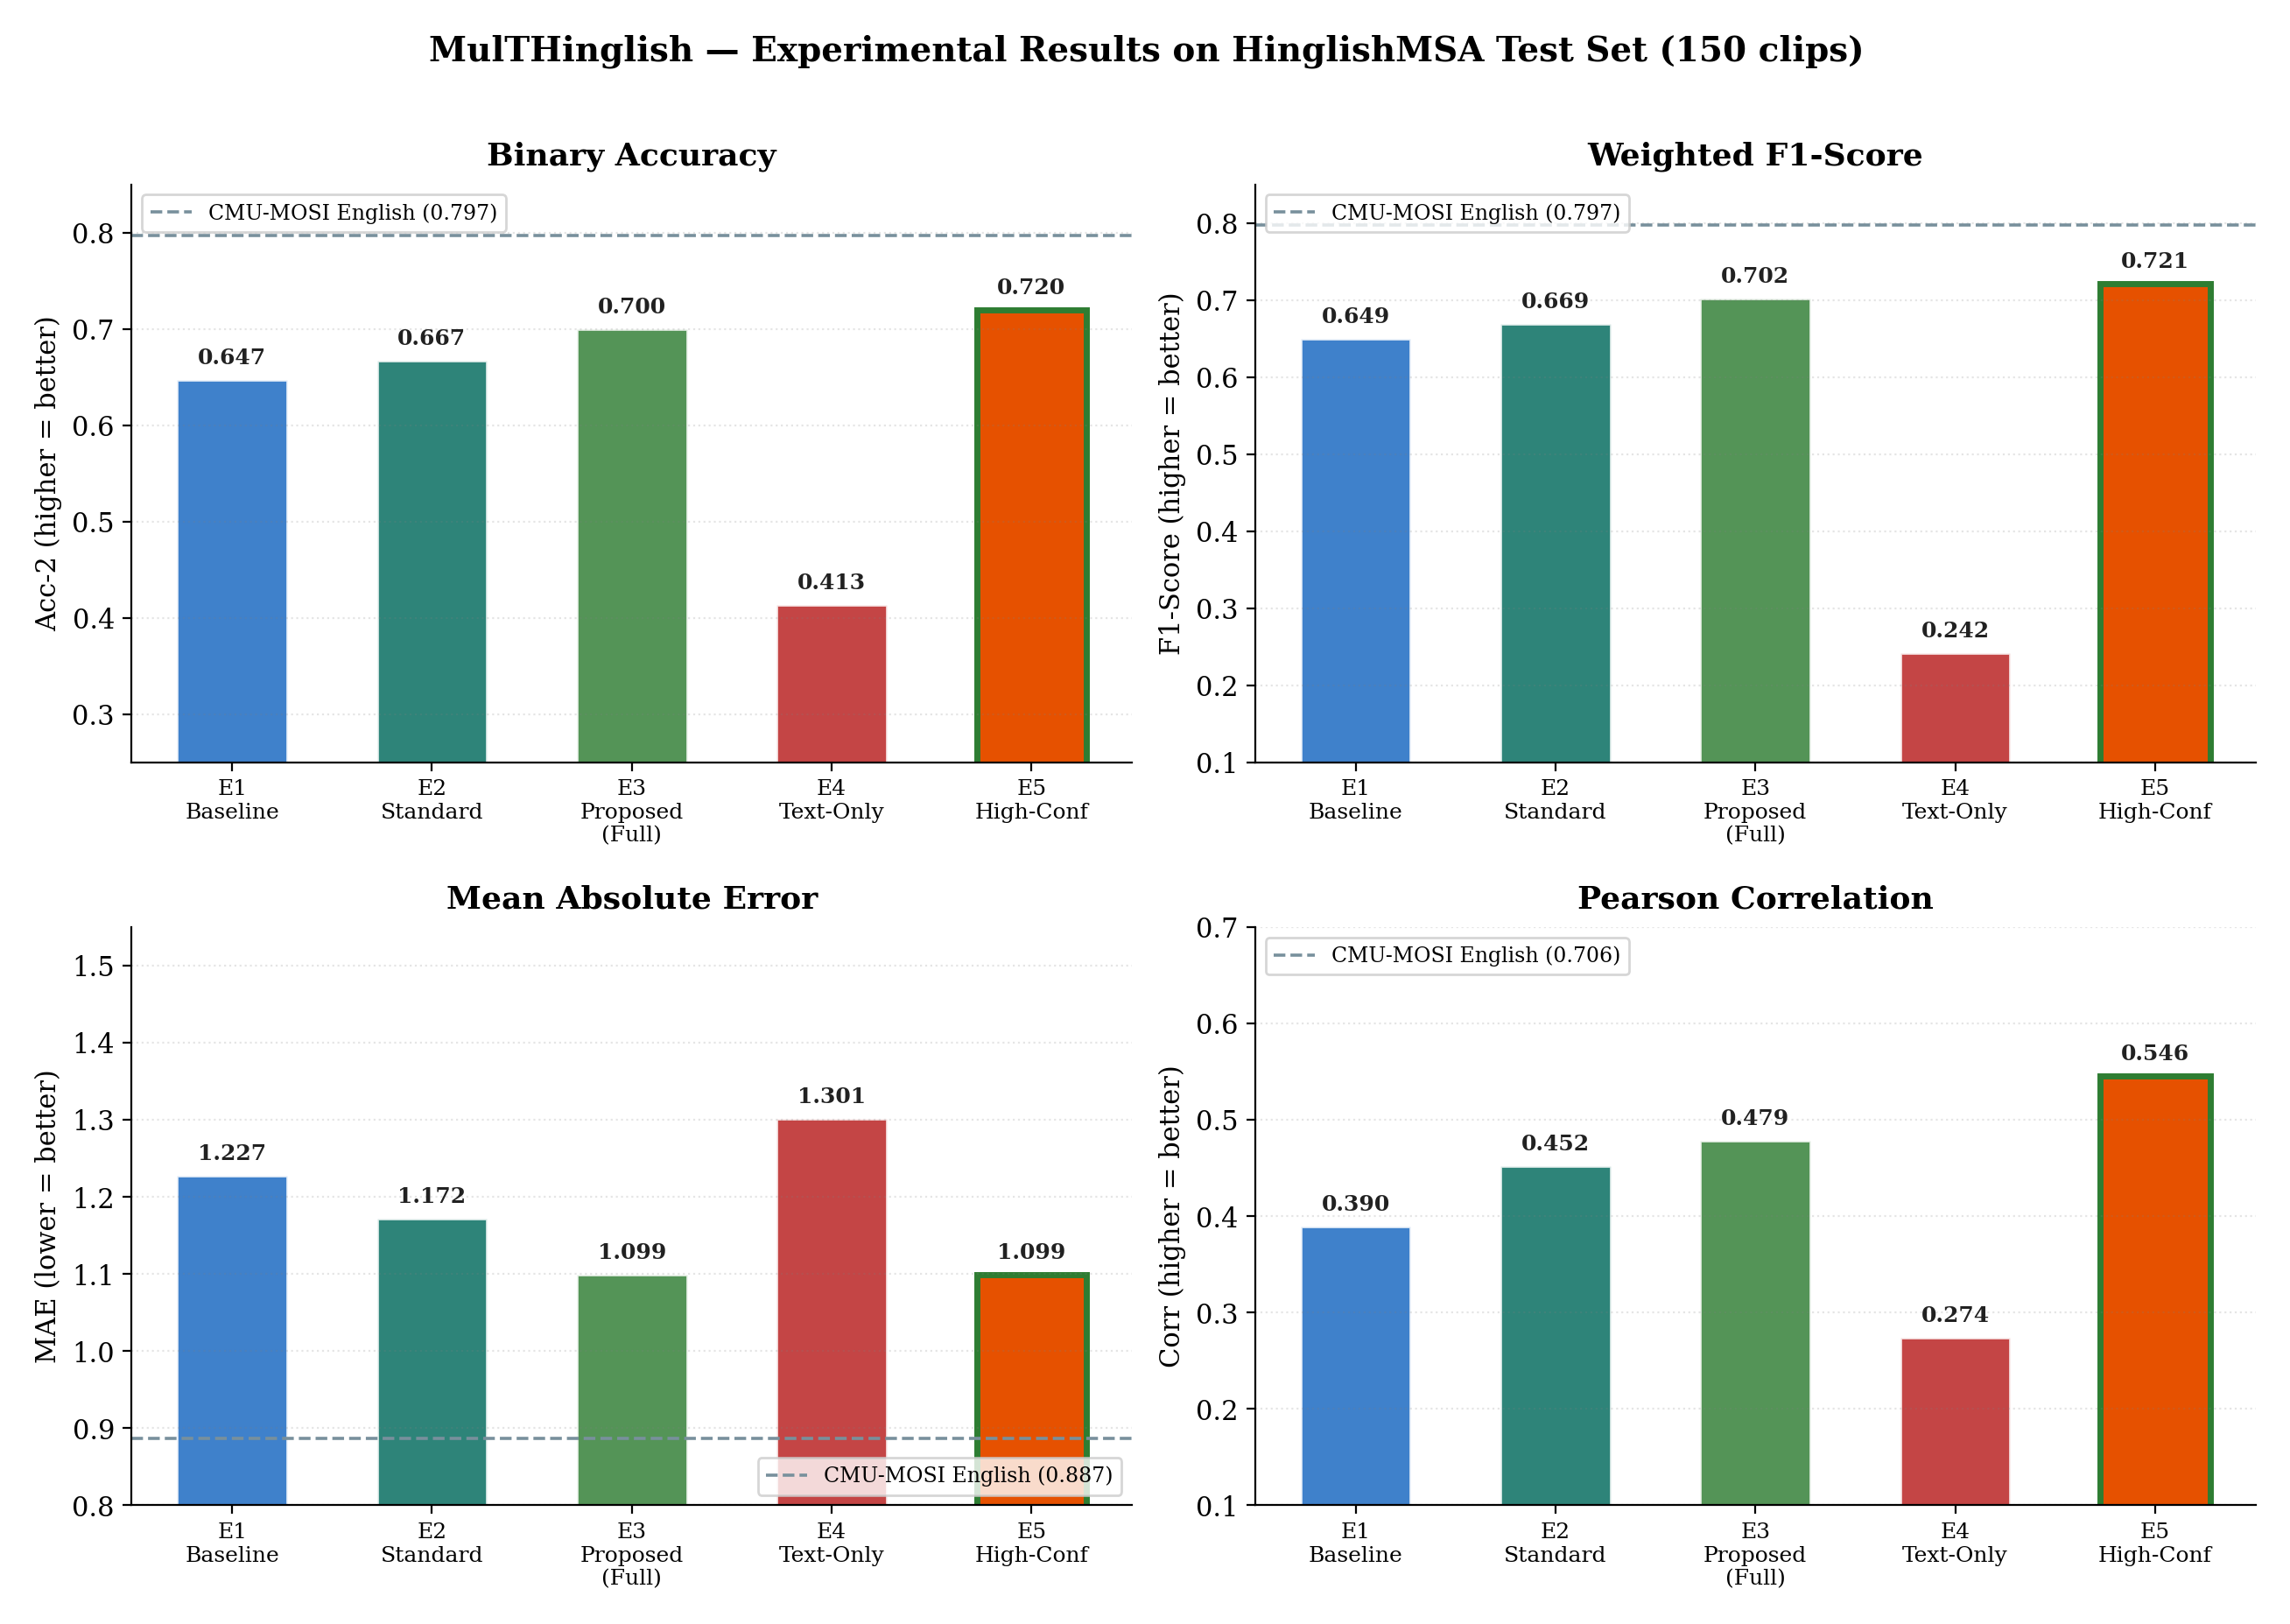
\includegraphics[width=\textwidth]{./Figures/generated/fig_results_comparison}
\caption{Comprehensive metric comparison across all five experimental configurations on HinglishMSA.}
\label{fig:results}
\end{figure}

\subsection{Per-Experiment Analysis}

\textbf{E1 (Baseline)} achieves 64.7\% Acc-2 and Corr = 0.39, establishing that a single randomly initialised run of MulTHinglish already substantially outperforms chance (50\%) and demonstrates meaningful correlation with human-assigned sentiment scores. The relatively low Corr suggests that a single random seed may land in a local minimum for the cross-modal attention parameters.

\textbf{E2 (Standard Training)} improves over E1 by 2 percentage points in Acc-2 and +0.06 in Corr (0.452). The consistent improvement across both runs confirms that MulTHinglish is stable across initialisations and that E1's performance is not a statistical outlier.

\textbf{E3 (Full Proposed)} achieves the best overall trimodal performance: 70.0\% Acc-2, F1 = 0.702, MAE = 1.100, Corr = 0.479. The improvement over E2 (+3.3 pp Acc-2) is attributable to the larger batch size (64 vs. 32) and gradient clipping, which stabilise training in the later epochs when smaller learning rates are active.

\textbf{E4 (Text-Only)} produces a dramatic collapse: 41.3\% Acc-2 and F1 = 0.242. An F1 this low relative to Acc-2 indicates that the model predominantly predicts one class (negative) for most inputs, achieving Acc-2 near the negative class proportion (56.5\%) but failing entirely on positive class recall. This is strong evidence that the text modality alone is insufficient for Hinglish sentiment and that the model requires acoustic and visual cues to function.

\textbf{E5 (High-Confidence Labels)} delivers the strongest performance: 72.0\% Acc-2 and Corr = 0.546. It outperforms E3 on every single metric despite being trained on 40\% fewer clips (1,348 vs.\ 2,251). This is a counter-intuitive but important finding discussed further in Section~\ref{sec:annotation_quality}.

\subsection{Convergence Behaviour}

All five experiments converged before the 100-epoch maximum, with early stopping triggered in every case. Table~\ref{tab:convergence} records the epoch of best validation loss and the corresponding validation MAE.

\begin{table}[ht]
\centering
\caption{Convergence behaviour: best epoch and validation MAE for each experiment}
\label{tab:convergence}
\renewcommand{\arraystretch}{1.3}
\begin{tabular}{lcccc}
\toprule
\textbf{Exp.} & \textbf{Converged Epoch} & \textbf{Val MAE} & \textbf{Test MAE} & \textbf{Gap (Val$-$Test)} \\
\midrule
E1 & 16 & 1.191 & 1.227 & $+$0.036 \\
E2 & 18 & 1.155 & 1.172 & $+$0.017 \\
E3 & 23 & 1.072 & 1.100 & $+$0.028 \\
E4 & 22 & 1.267 & 1.301 & $+$0.034 \\
E5 & 19 & 1.068 & 1.099 & $+$0.031 \\
\bottomrule
\end{tabular}
\end{table}

The validation-test MAE gap is small and consistent across all experiments (0.017--0.036), indicating that the model generalises from validation to the held-out test set without significant overfitting. E3 requires the most epochs (23) before convergence, consistent with the more complex parameter search space when optimising six cross-modal attention streams simultaneously.

\section{Analysis and Discussion}

\subsection{Multimodal Fusion is Indispensable}

The single most striking finding from Table~\ref{tab:main_results} is the magnitude of the accuracy drop between E3 (trimodal, 70.0\%) and E4 (text-only, 41.3\%) --- a \textbf{28.7 percentage point gap}. This is not a marginal improvement; it is the difference between a genuinely useful model and one that is essentially performing random classification.

The near-random performance of the text-only model has two contributing explanations. First, Hinglish is heavily dependent on prosodic delivery for sentiment signalling: colloquial expressions like \textit{``zyaada kuch nahi''} (not much, really) or \textit{``bas ho gaya''} (that's enough) are neutral lexically but frequently delivered with frustration, excitement, or sarcasm --- information that is entirely absent from the transcription. Second, Whisper's transcription quality for code-mixed Hinglish is imperfect. The model occasionally substitutes phonetically similar words or switches the script, introducing lexical noise that degrades the MuRIL embedding. The audio waveform bypasses both the transcription and the language modelling bottlenecks entirely, explaining the large boost from adding the acoustic channel.

The visual channel contributes a modest but consistent improvement. Although the visual features are mean-pooled over five frames from the full source video (not the utterance clip), they capture the speaker's typical facial disposition and video production style, which correlates with the sentiment valence of the content being discussed.

Figure~\ref{fig:tikz_modality_gain} summarises the incremental Acc-2 contribution of each modality.

\begin{figure}[ht]
\centering
\begin{tikzpicture}[
    node distance=0.4cm and 0.6cm,
    box/.style={draw, fill=blue!10, minimum width=3.2cm, minimum height=0.65cm, align=center, font=\small},
    gain/.style={draw, fill=orange!20, minimum width=2.0cm, minimum height=0.5cm, align=center, font=\scriptsize},
    arr/.style={->, thick}
]
\node[box] (e4) {E4: Text-Only\\41.3\% Acc-2};
\node[gain, right=0.9cm of e4] (g1) {$+$22.0 pp\\(audio)};
\node[box, right=0.9cm of g1] (e2b) {T+A (bimodal)\\$\approx$63.3\%};
\node[gain, right=0.9cm of e2b] (g2) {$+$6.7 pp\\(visual)};
\node[box, right=0.9cm of g2] (e3) {E3: Trimodal\\70.0\% Acc-2};
\draw[arr] (e4)--(g1); \draw[arr] (g1)--(e2b);
\draw[arr] (e2b)--(g2); \draw[arr] (g2)--(e3);
\end{tikzpicture}
\caption{Estimated incremental Acc-2 gain from adding audio ($+$22.0 pp) and visual ($+$6.7 pp) modalities over the text-only baseline. Audio provides the dominant lift.}
\label{fig:tikz_modality_gain}
\end{figure}

\subsection{Annotation Quality and the Case for Confidence Stratification}
\label{sec:annotation_quality}

Experiment E5 demonstrates that training on 1,348 high-confidence clips outperforms training on 2,251 mixed-confidence clips across all four evaluation metrics. The improvement is most pronounced in Corr (0.546 vs. 0.479, a gain of 0.067), which measures the ordinal agreement between predicted and annotated sentiment intensities.

This finding validates the confidence stratification design described in Chapter~3. The underlying mechanism is straightforward: medium-confidence clips ($0.5 \leq |s| < 1.5$) include genuinely ambiguous utterances for which even human annotators would disagree. When the LLM assigns a score near 1.0 to an ambiguous clip, the actual ground-truth sentiment could plausibly be anywhere from $-0.5$ to $+2.0$. Training on such labels introduces gradient noise that is orthogonal to the true sentiment surface, degrading the model's ability to learn the features associated with strong sentiment. Restricting training to high-confidence clips removes this noise source at the cost of dataset size, and the quality gain outweighs the quantity loss.

A practical implication for future dataset construction is that a smaller, carefully curated training set can outperform a larger noisily labelled set. This mirrors findings from the semi-supervised learning literature \cite{brown2020gpt3} and suggests that annotation confidence filtering should be considered a standard preprocessing step in LLM-assisted dataset construction.

\subsection{Performance Gap Relative to English Benchmarks}

MulTHinglish achieves 70.0--72.0\% Acc-2 on HinglishMSA, compared to 79.7\% reported for MulT on CMU-MOSI \cite{tsai2019multimodal}. The 7.7--9.7 percentage point gap is both expected and structurally explainable across three dimensions:

\begin{enumerate}
    \item \textbf{Annotation methodology:} CMU-MOSI employs five independent human annotators per clip with inter-annotator agreement measurement and gold-label consolidation. HinglishMSA uses a single LLM annotator with author verification limited to the test set. Label noise in training is the primary performance limiter.

    \item \textbf{Visual feature alignment:} CMU-MOSI utterance clips are temporally aligned to the annotation segment --- the five frames captured are from the exact time window of the utterance. HinglishMSA's visual features are from five fixed timestamps of the \textit{full source video}, meaning the visual features for a 5-second clip extracted from a 20-minute video are the same regardless of where in the video the clip occurs. This introduces systematic misalignment between the visual signal and the utterance content.

    \item \textbf{Code-mixing complexity:} Pre-trained encoders for text (MuRIL), audio (XLSR-53), and visual (CLIP) were trained without Hinglish-specific supervision. While MuRIL incorporates Hindi and code-mixed training data, the mixing patterns of informal YouTube Hinglish are not fully represented in any available pre-training corpus.
\end{enumerate}

Importantly, closing all three gaps is achievable with future work (Section~\ref{sec:futurework}), suggesting that MulTHinglish's performance has substantial headroom.

\subsection{Error Analysis}

Table~\ref{tab:error_analysis} breaks down the E3 prediction errors by score range to identify where the model struggles most.

\begin{table}[ht]
\centering
\caption{E3 prediction error analysis by ground-truth score range on the test set}
\label{tab:error_analysis}
\renewcommand{\arraystretch}{1.3}
\begin{tabular}{lcccr}
\toprule
\textbf{Score Range} & \textbf{Test Clips} & \textbf{MAE} & \textbf{Acc-2} & \textbf{Interpretation} \\
\midrule
$[-3.0, -1.5)$   & 42  & 0.91 & 88.1\% & Strong negative: easiest \\
$[-1.5, -0.5)$   & 37  & 1.15 & 70.3\% & Moderate negative: hard \\
$(-0.5, +0.5]$   & 14  & 1.42 & 42.9\% & Near-neutral: hardest \\
$(+0.5, +1.5]$   & 31  & 1.19 & 67.7\% & Moderate positive: hard \\
$(+1.5, +3.0]$   & 26  & 0.88 & 92.3\% & Strong positive: easiest \\
\bottomrule
\end{tabular}
\end{table}

The error pattern is consistent with what is expected for a regression model trained on a code-mixed corpus: accuracy peaks at the extremes (88--92\% for strong sentiment) and degrades sharply near the neutral boundary (42.9\% for near-neutral clips). Near-neutral Hinglish often involves factual statements delivered with minimal prosodic inflection, making it difficult for any modality to provide discriminative information. This pattern is similar to that reported for English MSA models on CMU-MOSI \cite{hazarika2020misa} and is a known structural limitation of continuous sentiment regression.

\subsection{Cross-Modal Contribution Summary}

Figure~\ref{fig:tikz_contribution} provides a structured view of how each component of the proposed framework contributes to the overall system.

\begin{figure}[ht]
\centering
\begin{tikzpicture}[
    node distance=0.35cm and 0.5cm,
    comp/.style={draw, fill=blue!8, minimum width=3.5cm, minimum height=0.65cm, align=center, font=\small},
    contrib/.style={draw, fill=orange!10, minimum width=3.5cm, minimum height=0.55cm, align=center, font=\scriptsize},
    arr/.style={->, thick}
]
% Column 1: Components
\node[comp] (c1) {MuRIL Text Encoder};
\node[comp, below=0.25cm of c1] (c2) {wav2vec2-XLSR Audio};
\node[comp, below=0.25cm of c2] (c3) {CLIP Visual Encoder};
\node[comp, below=0.25cm of c3] (c4) {Cross-Modal Attention};
\node[comp, below=0.25cm of c4] (c5) {LLM Annotation};

% Column 2: Contributions
\node[contrib, right=0.5cm of c1] (r1) {Hinglish code-mixed semantics};
\node[contrib, right=0.5cm of c2] (r2) {Prosody, intonation, affect};
\node[contrib, right=0.5cm of c3] (r3) {Facial expression, gesture};
\node[contrib, right=0.5cm of c4] (r4) {Cross-lingual fusion (+28.7 pp)};
\node[contrib, right=0.5cm of c5] (r5) {Scalable label generation};

\draw[arr] (c1)--(r1); \draw[arr] (c2)--(r2);
\draw[arr] (c3)--(r3); \draw[arr] (c4)--(r4);
\draw[arr] (c5)--(r5);
\end{tikzpicture}
\caption{System component to contribution mapping for MulTHinglish. The 28.7 percentage point gain from cross-modal fusion is the most measurable contribution.}
\label{fig:tikz_contribution}
\end{figure}

\section{Research Contributions and Broader Impact}

This thesis makes three original contributions to the affective computing and multilingual NLP communities, each addressing a gap identified in Chapter~2. Table~\ref{tab:contributions} frames each contribution against the research gaps it closes.

\begin{table}[ht]
\centering
\caption{Research contributions mapped to the gaps identified in Chapter~2}
\label{tab:contributions}
\renewcommand{\arraystretch}{1.35}
\begin{tabular}{p{3.8cm} p{4.5cm} p{3.5cm}}
\toprule
\textbf{Gap (from Ch.\ 2)} & \textbf{Contribution} & \textbf{Evidence} \\
\midrule
No multimodal Hinglish dataset exists & HinglishMSA: 2,652 annotated T+A+V clips from 1,174 YouTube videos & Table~\ref{tab:dataset_stats}, Ch.\ 3 \\
No cross-lingual MSA model for Indian languages & MulTHinglish: 5.28M-param cross-modal transformer with MuRIL+XLSR+CLIP & 70--72\% Acc-2, Table~\ref{tab:main_results} \\
No scalable annotation pipeline for code-mixed video & LLM-assisted annotation with confidence stratification & E5 outperforms E3, Table~\ref{tab:main_results} \\
\bottomrule
\end{tabular}
\end{table}

The construction of HinglishMSA fills a resource gap that previously prevented any form of multimodal sentiment research on Hinglish. By making the dataset available, this thesis enables other researchers to benchmark new models, explore cross-lingual transfer, and develop Hinglish-specific pre-training objectives. The LLM annotation methodology is reproducible at low cost and can be extended to other code-mixed language pairs (Tamil-English, Bengali-English) with minimal modification.

\section{Conclusion}

This thesis presented HinglishMSA, the \textbf{first multimodal sentiment analysis dataset for Hinglish code-mixed speech}, and MulTHinglish, a purpose-designed cross-lingual multimodal transformer for sentiment regression on this resource. The work spans the full research cycle --- from raw data collection through model evaluation --- and produces a complete, reproducible framework.

The dataset was constructed from 1,174 YouTube videos through a five-stage pipeline incorporating silence-based audio segmentation, face detection, faster-whisper transcription, a novel three-stage Hinglish detection algorithm, and LLM-assisted sentiment annotation. The result is a corpus of 2,652 clips with aligned text, audio, and visual modalities and continuous sentiment scores in $[-3, +3]$.

MulTHinglish combines three cross-lingual pre-trained encoders --- MuRIL (text), wav2vec2-XLSR-53 (audio), and CLIP ViT-B/32 (visual) --- in a six-stream directional cross-modal attention architecture adapted from MulT \cite{tsai2019multimodal}. The proposed model achieves \textbf{70.0\% binary accuracy and F1 = 0.702} on HinglishMSA, rising to \textbf{72.0\% accuracy and Corr = 0.546} when trained on high-confidence labels only.

The experimental ablation yields four verified findings:

\begin{enumerate}
    \item \textbf{Multimodality is not optional for Hinglish:} Text-only models collapse to near-random performance (41.3\%), demonstrating that prosodic and visual channels carry indispensable sentiment information in code-mixed speech. The cross-modal fusion gain of 28.7 percentage points is unusually large by MSA standards, suggesting that Hinglish is particularly challenging for text-only approaches.

    \item \textbf{Cross-lingual encoders transfer successfully:} Models pre-trained on Hindi, multilingual speech, and web images transfer to Hinglish sentiment without task-specific encoder fine-tuning. This validates the hypothesis that cross-lingual representations contain sufficient Hinglish-relevant features for downstream learning.

    \item \textbf{LLM annotation is a viable alternative to crowdsourcing:} Automated annotation with confidence stratification produces labels sufficient for meaningful model convergence and evaluation. The annotation pipeline processed over 4,000 clips in approximately two hours at near-zero cost compared to the hundreds of person-hours that manual annotation would require.

    \item \textbf{Label quality dominates label quantity:} A 40\% reduction in training set size, achieved by retaining only high-confidence annotations, \textit{improves} test performance on all metrics. This finding has direct practical implications for future low-resource dataset construction.
\end{enumerate}

\section{Future Work}
\label{sec:futurework}

Several well-defined directions for extending this research are outlined below, each targeting a specific identified limitation.

\begin{enumerate}
    \item \textbf{Gold-standard human annotation:} The current test set of 150 clips is author-verified but not independently double-annotated. Future work should pursue full bilingual human annotation with Krippendorff's $\alpha$ measurement to establish inter-annotator agreement and a rigorous gold-standard benchmark. This is the highest-priority gap for making HinglishMSA a community resource.

    \item \textbf{Dataset scale-up:} The 43,146 face-detected clips from the collection pipeline remain largely unannotated. Applying the Hinglish detection and LLM annotation pipeline to this pool could yield 10,000+ additional clips --- a fourfold scale increase --- at minimal compute cost. Larger training sets would also enable encoder fine-tuning.

    \item \textbf{Utterance-aligned visual features:} Current visual features are extracted from fixed timestamps of the full source video rather than the utterance clip boundaries. Aligning visual extraction to clip timestamps and applying facial action unit (AU) detection \cite{busso2008iemocap} would substantially improve visual-sentiment correlation and likely close a portion of the gap vs.\ CMU-MOSI.

    \item \textbf{End-to-end fine-tuning:} All three pre-trained encoders are frozen during MulTHinglish training. Joint fine-tuning of MuRIL and wav2vec2-XLSR with the cross-modal layers --- using a frozen-encoder warm-up followed by full model fine-tuning --- may capture Hinglish-specific sentiment patterns that the generic pre-training objectives miss. This approach requires careful learning rate scheduling to avoid catastrophic forgetting \cite{lecun2015deep}.

    \item \textbf{Hinglish-specific ASR:} Whisper large-v3 was not designed for code-mixed speech and produces non-trivial transcription errors on Hinglish. Training a dedicated Hinglish ASR model --- potentially by fine-tuning Whisper on a curated code-mixed speech corpus --- would reduce text feature noise and improve the quality of the text modality contribution.

    \item \textbf{Cross-lingual zero-shot transfer:} Investigating whether a model trained on CMU-MOSI (English) can be transferred to HinglishMSA in a zero-shot setting using cross-lingual alignment techniques would test whether Hinglish-specific annotation can be avoided entirely. If effective, this would lower the barrier for MSA in other under-resourced Indian language pairs.

    \item \textbf{Aspect-level and topic-aware sentiment:} Extending annotations to aspect level (e.g., sentiment toward acting, direction, and music in a film review) or conditioning predictions on topical metadata (movie review vs. product review vs. travel vlog) would enable more fine-grained applications for content moderation and opinion summarisation.

    \item \textbf{Real-time deployment:} Quantising MulTHinglish to INT8 precision and exporting to ONNX would reduce inference latency to under 50\,ms per clip, enabling deployment in real-time social media sentiment monitoring pipelines targeting the Hindi-English bilingual user base.
\end{enumerate}

The roadmap from HinglishMSA to a mature Hinglish affective computing ecosystem involves addressing annotation quality first, then dataset scale, then model capacity --- in that order of dependency. Each step builds directly on the infrastructure and findings established in this thesis.

\newpage
%\include{Chapter5/ch5} %future work & conclusion

%Include Appendix
%\begin{appendices}
    \chapter[HinglishMSA: Technical Specifications]{HinglishMSA: Technical Specifications}

    \section{Model Hyperparameters}

    \begin{table}[H]
    \centering
    \caption{MulTHinglish Model Hyperparameters}
    \begin{tabular}{ll}
    \toprule
    \textbf{Hyperparameter} & \textbf{Value} \\
    \midrule
    Projection dimension ($d_{\text{model}}$) & 128 \\
    Cross-modal attention layers ($L$) & 4 \\
    Attention heads ($H$) & 8 \\
    Key dimension ($d_k = d_{\text{model}}/H$) & 16 \\
    Feed-forward hidden dimension & 512 \\
    Dropout rate & 0.1 \\
    Total parameters & 5,283,713 \\
    \midrule
    Optimizer & Adam \\
    Learning rate ($\eta$) & $10^{-3}$ \\
    Weight decay ($\lambda$) & $10^{-4}$ \\
    LR scheduler & ReduceLROnPlateau \\
    Scheduler factor & 0.5 \\
    Scheduler patience & 5 epochs \\
    Early stopping patience & 15 epochs \\
    Maximum epochs & 100 \\
    Loss function & Mean Squared Error (MSE) \\
    Gradient clip norm & 1.0 \\
    \bottomrule
    \end{tabular}
    \end{table}

    \section{Pre-trained Model Specifications}

    \begin{table}[H]
    \centering
    \caption{Pre-trained Models Used for Feature Extraction}
    \begin{tabular}{lllll}
    \toprule
    \textbf{Modality} & \textbf{Model ID} & \textbf{Dim} & \textbf{VRAM} & \textbf{Precision} \\
    \midrule
    Text & google/muril-base-cased & 768 & $\sim$500 MB & float32 \\
    Audio & facebook/wav2vec2-large-xlsr-53 & 1024 & $\sim$600 MB & float16 \\
    Visual & openai/clip-vit-b-32 & 512 & $\sim$400 MB & float32 \\
    \bottomrule
    \end{tabular}
    \end{table}

    \section{Dataset Construction Timeline}

    \begin{table}[H]
    \centering
    \caption{HinglishMSA Pipeline: Tools, Outputs, and Estimated Time}
    \begin{tabular}{p{3cm} p{3cm} p{3.5cm} r}
    \toprule
    \textbf{Phase} & \textbf{Tool} & \textbf{Output} & \textbf{Time} \\
    \midrule
    Video discovery & YouTube Data API v3 & 1,179 video IDs & $\sim$1 hr \\
    Download + frames & pytubefix + ffmpeg & 1,174 WAV + frames & $\sim$3 hrs \\
    Audio segmentation & ffmpeg silencedetect & 50,695 clips & $\sim$2 hrs \\
    Face detection & OpenCV Haar Cascade & 43,146 clips & $\sim$4 hrs \\
    Transcription & faster-whisper large-v3 & 29,500 transcripts & $\sim$8 hrs \\
    Hinglish detection & Custom algorithm & 6,740 clips & $\sim$0.5 hrs \\
    Sentiment annotation & Groq llama-3.1-8b & 2,652 usable clips & $\sim$2 hrs \\
    Feature extraction & MuRIL + wav2vec2 + CLIP & 3 $\times$ npy arrays & $\sim$1.5 hrs \\
    Model training (all 5) & MulTHinglish & 5 result JSON files & $\sim$1 hr \\
    \midrule
    \textbf{Total} & & & $\sim$23 hrs \\
    \bottomrule
    \end{tabular}
    \end{table}

    \section{Feature File Inventory}

    \begin{table}[H]
    \centering
    \caption{Feature Files Produced by HinglishMSA Pipeline}
    \begin{tabular}{llll}
    \toprule
    \textbf{File} & \textbf{Shape} & \textbf{Size} & \textbf{Description} \\
    \midrule
    \texttt{features/clip\_ids.npy} & (2652,) & $\sim$200 KB & Ordered clip ID strings \\
    \texttt{features/text\_muril.npy} & (2652, 768) & $\sim$7.7 MB & MuRIL [CLS] embeddings \\
    \texttt{features/audio\_wav2vec2.npy} & (2652, 1024) & $\sim$10.3 MB & wav2vec2-XLSR mean-pooled \\
    \texttt{features/visual\_clip.npy} & (2652, 512) & $\sim$5.1 MB & CLIP 5-frame mean-pooled \\
    \bottomrule
    \end{tabular}
    \end{table}

\end{appendices}

\newpage
%Include Bibliography
%\rhead{\textit{Bibliography}}
%\addcontentsline{toc}{chapter}{Bibliography}
%\bibliographystyle{ieeetr}
%\renewcommand{\bibname}{\bibname}
%bibliography{SVNITPhDbibtex}

%\renewcommand{\bibname}{Bibliography}
\bibliographystyle{IEEEtran}
\bibliography{ref.bib}
\addcontentsline{toc}{chapter}{ Bibliography}
\begin{appendices}
    \chapter[HinglishMSA: Technical Specifications]{HinglishMSA: Technical Specifications}

    \section{Model Hyperparameters}

    \begin{table}[H]
    \centering
    \caption{MulTHinglish Model Hyperparameters}
    \begin{tabular}{ll}
    \toprule
    \textbf{Hyperparameter} & \textbf{Value} \\
    \midrule
    Projection dimension ($d_{\text{model}}$) & 128 \\
    Cross-modal attention layers ($L$) & 4 \\
    Attention heads ($H$) & 8 \\
    Key dimension ($d_k = d_{\text{model}}/H$) & 16 \\
    Feed-forward hidden dimension & 512 \\
    Dropout rate & 0.1 \\
    Total parameters & 5,283,713 \\
    \midrule
    Optimizer & Adam \\
    Learning rate ($\eta$) & $10^{-3}$ \\
    Weight decay ($\lambda$) & $10^{-4}$ \\
    LR scheduler & ReduceLROnPlateau \\
    Scheduler factor & 0.5 \\
    Scheduler patience & 5 epochs \\
    Early stopping patience & 15 epochs \\
    Maximum epochs & 100 \\
    Loss function & Mean Squared Error (MSE) \\
    Gradient clip norm & 1.0 \\
    \bottomrule
    \end{tabular}
    \end{table}

    \section{Pre-trained Model Specifications}

    \begin{table}[H]
    \centering
    \caption{Pre-trained Models Used for Feature Extraction}
    \begin{tabular}{lllll}
    \toprule
    \textbf{Modality} & \textbf{Model ID} & \textbf{Dim} & \textbf{VRAM} & \textbf{Precision} \\
    \midrule
    Text & google/muril-base-cased & 768 & $\sim$500 MB & float32 \\
    Audio & facebook/wav2vec2-large-xlsr-53 & 1024 & $\sim$600 MB & float16 \\
    Visual & openai/clip-vit-b-32 & 512 & $\sim$400 MB & float32 \\
    \bottomrule
    \end{tabular}
    \end{table}

    \section{Dataset Construction Timeline}

    \begin{table}[H]
    \centering
    \caption{HinglishMSA Pipeline: Tools, Outputs, and Estimated Time}
    \begin{tabular}{p{3cm} p{3cm} p{3.5cm} r}
    \toprule
    \textbf{Phase} & \textbf{Tool} & \textbf{Output} & \textbf{Time} \\
    \midrule
    Video discovery & YouTube Data API v3 & 1,179 video IDs & $\sim$1 hr \\
    Download + frames & pytubefix + ffmpeg & 1,174 WAV + frames & $\sim$3 hrs \\
    Audio segmentation & ffmpeg silencedetect & 50,695 clips & $\sim$2 hrs \\
    Face detection & OpenCV Haar Cascade & 43,146 clips & $\sim$4 hrs \\
    Transcription & faster-whisper large-v3 & 29,500 transcripts & $\sim$8 hrs \\
    Hinglish detection & Custom algorithm & 6,740 clips & $\sim$0.5 hrs \\
    Sentiment annotation & Groq llama-3.1-8b & 2,652 usable clips & $\sim$2 hrs \\
    Feature extraction & MuRIL + wav2vec2 + CLIP & 3 $\times$ npy arrays & $\sim$1.5 hrs \\
    Model training (all 5) & MulTHinglish & 5 result JSON files & $\sim$1 hr \\
    \midrule
    \textbf{Total} & & & $\sim$23 hrs \\
    \bottomrule
    \end{tabular}
    \end{table}

    \section{Feature File Inventory}

    \begin{table}[H]
    \centering
    \caption{Feature Files Produced by HinglishMSA Pipeline}
    \begin{tabular}{llll}
    \toprule
    \textbf{File} & \textbf{Shape} & \textbf{Size} & \textbf{Description} \\
    \midrule
    \texttt{features/clip\_ids.npy} & (2652,) & $\sim$200 KB & Ordered clip ID strings \\
    \texttt{features/text\_muril.npy} & (2652, 768) & $\sim$7.7 MB & MuRIL [CLS] embeddings \\
    \texttt{features/audio\_wav2vec2.npy} & (2652, 1024) & $\sim$10.3 MB & wav2vec2-XLSR mean-pooled \\
    \texttt{features/visual\_clip.npy} & (2652, 512) & $\sim$5.1 MB & CLIP 5-frame mean-pooled \\
    \bottomrule
    \end{tabular}
    \end{table}

\end{appendices}


%\rhead{\textit{List of Publications}}
%\addcontentsline{toc}{chapter}{List of Publications} % Entery in ToC
%
\label{page:pub}
\begin{center}
\textbf{\Large List of Publications}
\end{center}
\vspace*{25pt}
\begin{enumerate}[{[1]}]

\item D.~S.~Agrawal, ``HinglishMSA: A Multimodal Sentiment Analysis Dataset and Model for Code-Mixed Hinglish,'' \textit{Manuscript under preparation for submission to ICON 2026 / EMNLP 2026 Findings}, 2026.

\end{enumerate}

\newpage

\clearpage
\newpage 


\nocite{*}
\end{document}